\chapterimage{Pictures/chap02/dof-dragons-848.png}

\chapter{几何与变换}\label{chap:几何与变换}
\setcounter{sidenote}{1}

几乎所有非平凡\sidenote{译者注:原文nontrivial。}的图形程序都建立在几何类的基础上。
这些类表示数学概念例如点、向量以及射线。
因为这些类贯穿了整个系统,所以良好的抽象和高效的实现至关重要。
本章介绍了pbrt几何基础的接口和实现。
注意这些并不是表示实际场景几何体的类(三角形、球体等);
那些类是第\refchap{形状}的主题。

本章几何类在pbrt发行版的文件
\href{https://github.com/mmp/pbrt-v3/tree/master/src/core/geometry.h}{\ttfamily core/geometry.h}
和\href{https://github.com/mmp/pbrt-v3/tree/master/src/core/geometry.cpp}{\ttfamily core/geometry.cpp}
中定义,变换矩阵(\refsec{变换})在文件
\href{https://github.com/mmp/pbrt-v3/tree/master/src/core/transform.h}{\ttfamily core/transform.h}和
\href{https://github.com/mmp/pbrt-v3/tree/master/src/core/transform.cpp}{\ttfamily core/transform.cpp}
中实现。

\section{坐标系统}\label{sec:坐标系统}

按计算机图形学中的经典做法,
pbrt用三个坐标值$x,y$和$z$表示\keyindex{点}{point}{}、
\keyindex{向量}{vector}{}和\keyindex{法向量}{normal vector}{vector向量}。
这些值须在\keyindex{坐标系统}{coordinate system}{}下才有意义,
即定义了空间的原点并给出三个线性独立的向量定义$x,y$和$z$坐标轴。
总之,定义了坐标系的原点和三个向量称为\keyindex{坐标系}{frame}{}。
给定3D中的任意一点或方向,其$(x,y,z)$坐标值取决于它和坐标系的关系。
\reffig{2.1}以2D形式给出例子说明了这点。
\begin{figure}
    %LaTeX with PSTricks extensions
%%Creator: Inkscape 1.0.1 (3bc2e813f5, 2020-09-07)
%%Please note this file requires PSTricks extensions
\psset{xunit=.5pt,yunit=.5pt,runit=.5pt}
\begin{pspicture}(327.3999939,474.47000122)
{
\newrgbcolor{curcolor}{0 0 0}
\pscustom[linewidth=1,linecolor=curcolor]
{
\newpath
\moveto(5.5,318.58000122)
\lineto(5.5,38.68000122)
\lineto(286.4,38.68000122)
}
}
{
\newrgbcolor{curcolor}{0 0 0}
\pscustom[linestyle=none,fillstyle=solid,fillcolor=curcolor]
{
\newpath
\moveto(0,313.67000122)
\lineto(5.5,317.93000122)
\lineto(11.01,313.67000122)
\lineto(5.5,326.68000122)
\closepath
}
}
{
\newrgbcolor{curcolor}{0.65098041 0.65098041 0.65098041}
\pscustom[linestyle=none,fillstyle=solid,fillcolor=curcolor]
{
\newpath
\moveto(1.2,315.22000122)
\lineto(5.5,325.37000122)
\lineto(5.5,318.56000122)
\closepath
}
}
{
\newrgbcolor{curcolor}{0.40000001 0.40000001 0.40000001}
\pscustom[linestyle=none,fillstyle=solid,fillcolor=curcolor]
{
\newpath
\moveto(9.8,315.22000122)
\lineto(5.5,325.37000122)
\lineto(5.5,318.56000122)
\closepath
}
}
{
\newrgbcolor{curcolor}{0 0 0}
\pscustom[linestyle=none,fillstyle=solid,fillcolor=curcolor]
{
\newpath
\moveto(281.49,33.18000122)
\lineto(285.75,38.68000122)
\lineto(281.49,44.18000122)
\lineto(294.5,38.68000122)
\closepath
}
}
{
\newrgbcolor{curcolor}{0.65098041 0.65098041 0.65098041}
\pscustom[linestyle=none,fillstyle=solid,fillcolor=curcolor]
{
\newpath
\moveto(283.05,34.38000122)
\lineto(293.19,38.68000122)
\lineto(286.38,38.68000122)
\closepath
}
}
{
\newrgbcolor{curcolor}{0.40000001 0.40000001 0.40000001}
\pscustom[linestyle=none,fillstyle=solid,fillcolor=curcolor]
{
\newpath
\moveto(283.05,42.98000122)
\lineto(293.19,38.68000122)
\lineto(286.38,38.68000122)
\closepath
}
}
{
\newrgbcolor{curcolor}{0 0 0}
\pscustom[linestyle=none,fillstyle=solid,fillcolor=curcolor]
{
\newpath
\moveto(219,243.68000793)
\curveto(219,249.91677562)(211.46003012,253.03903011)(207.05050397,248.62950396)
\curveto(202.64097782,244.21997781)(205.76323232,236.68000793)(212,236.68000793)
\curveto(218.23676768,236.68000793)(221.35902218,244.21997781)(216.94949603,248.62950396)
\curveto(212.53996988,253.03903011)(205,249.91677562)(205,243.68000793)
\curveto(205,237.44324025)(212.53996988,234.32098576)(216.94949603,238.73051191)
\curveto(221.35902218,243.14003806)(218.23676768,250.68000793)(212,250.68000793)
\curveto(205.76323232,250.68000793)(202.64097782,243.14003806)(207.05050397,238.73051191)
\curveto(211.46003012,234.32098576)(219,237.44324025)(219,243.68000793)
\closepath
}
}
{
\newrgbcolor{curcolor}{0 0 0}
\pscustom[linewidth=1,linecolor=curcolor]
{
\newpath
\moveto(219,243.68000793)
\curveto(219,249.91677562)(211.46003012,253.03903011)(207.05050397,248.62950396)
\curveto(202.64097782,244.21997781)(205.76323232,236.68000793)(212,236.68000793)
\curveto(218.23676768,236.68000793)(221.35902218,244.21997781)(216.94949603,248.62950396)
\curveto(212.53996988,253.03903011)(205,249.91677562)(205,243.68000793)
\curveto(205,237.44324025)(212.53996988,234.32098576)(216.94949603,238.73051191)
\curveto(221.35902218,243.14003806)(218.23676768,250.68000793)(212,250.68000793)
\curveto(205.76323232,250.68000793)(202.64097782,243.14003806)(207.05050397,238.73051191)
\curveto(211.46003012,234.32098576)(219,237.44324025)(219,243.68000793)
\closepath
}
}
{
\newrgbcolor{curcolor}{0 0 0}
\pscustom[linewidth=0.5,linecolor=curcolor]
{
\newpath
\moveto(212.5,38.29998779)
\lineto(212.5,243.68000793)
}
}
{
\newrgbcolor{curcolor}{0 0 0}
\pscustom[linewidth=0.5,linecolor=curcolor]
{
\newpath
\moveto(212.5,36.30000122)
\lineto(212.5,26.33000122)
\lineto(5.56,26.33000122)
\lineto(5.56,36.30000122)
}
}
{
\newrgbcolor{curcolor}{0 0 0}
\pscustom[linewidth=1,linecolor=curcolor,linestyle=dashed,dash=4 4]
{
\newpath
\moveto(257.15,467.24000122)
\lineto(197.77,349.88000122)
\lineto(193.09,340.62000122)
\lineto(320.17,276.32000122)
}
}
{
\newrgbcolor{curcolor}{0 0 0}
\pscustom[linestyle=none,fillstyle=solid,fillcolor=curcolor]
{
\newpath
\moveto(250.02,465.34000122)
\lineto(256.85,466.66000122)
\lineto(259.84,460.37000122)
\lineto(260.81,474.47000122)
\closepath
}
}
{
\newrgbcolor{curcolor}{0.65098041 0.65098041 0.65098041}
\pscustom[linestyle=none,fillstyle=solid,fillcolor=curcolor]
{
\newpath
\moveto(251.8,466.19000122)
\lineto(260.21,473.30000122)
\lineto(257.14,467.22000122)
\closepath
}
}
{
\newrgbcolor{curcolor}{0.40000001 0.40000001 0.40000001}
\pscustom[linestyle=none,fillstyle=solid,fillcolor=curcolor]
{
\newpath
\moveto(259.47,462.31000122)
\lineto(260.21,473.30000122)
\lineto(257.14,467.22000122)
\closepath
}
}
{
\newrgbcolor{curcolor}{0 0 0}
\pscustom[linestyle=none,fillstyle=solid,fillcolor=curcolor]
{
\newpath
\moveto(313.31,273.63000122)
\lineto(319.59,276.61000122)
\lineto(318.27,283.45000122)
\lineto(327.4,272.66000122)
\closepath
}
}
{
\newrgbcolor{curcolor}{0.65098041 0.65098041 0.65098041}
\pscustom[linestyle=none,fillstyle=solid,fillcolor=curcolor]
{
\newpath
\moveto(315.24,274.00000122)
\lineto(326.23,273.25000122)
\lineto(320.15,276.33000122)
\closepath
}
}
{
\newrgbcolor{curcolor}{0.40000001 0.40000001 0.40000001}
\pscustom[linestyle=none,fillstyle=solid,fillcolor=curcolor]
{
\newpath
\moveto(319.12,281.67000122)
\lineto(326.23,273.25000122)
\lineto(320.15,276.33000122)
\closepath
}
}
{
\newrgbcolor{curcolor}{0 0 0}
\pscustom[linewidth=1,linecolor=curcolor]
{
\newpath
\moveto(215.15,249.80000122)
\lineto(251.83,322.30000122)
\lineto(197.77,349.88000122)
}
}
{
\newrgbcolor{curcolor}{0 0 0}
\pscustom[linestyle=none,fillstyle=solid,fillcolor=curcolor]
{
\newpath
\moveto(183.85300767,237.52316943)
\curveto(183.78504651,237.21734418)(183.75106592,237.1833636)(183.71708534,237.14938301)
\curveto(183.61514359,237.11540243)(183.37727951,237.11540243)(183.17339602,237.11540243)
\curveto(182.7996096,237.11540243)(182.39184261,237.11540243)(182.39184261,236.50375194)
\curveto(182.39184261,236.26588786)(182.59572611,236.09598495)(182.83359019,236.09598495)
\curveto(183.44524068,236.09598495)(184.15883292,236.16394611)(184.80446399,236.16394611)
\curveto(185.5860174,236.16394611)(186.40155138,236.09598495)(187.1491242,236.09598495)
\curveto(187.28504654,236.09598495)(187.69281353,236.09598495)(187.69281353,236.74161602)
\curveto(187.69281353,237.11540243)(187.3530077,237.11540243)(187.1491242,237.11540243)
\curveto(186.84329896,237.11540243)(186.46951255,237.11540243)(186.19766789,237.14938301)
\lineto(187.1491242,240.92122771)
\curveto(187.45494945,240.61540246)(188.16854169,240.1396743)(189.3238815,240.1396743)
\curveto(193.0957262,240.1396743)(195.44038641,243.57171317)(195.44038641,246.52802387)
\curveto(195.44038641,249.21248991)(193.43553203,250.09598507)(191.63456114,250.09598507)
\curveto(190.10543491,250.09598507)(188.98407568,249.2464705)(188.64426985,248.94064525)
\curveto(187.79475528,250.09598507)(186.3675708,250.09598507)(186.12970672,250.09598507)
\curveto(185.34815332,250.09598507)(184.70252224,249.65423749)(184.26077467,248.87268408)
\curveto(183.71708534,247.98918893)(183.4112601,246.83384912)(183.4112601,246.73190737)
\curveto(183.4112601,246.42608212)(183.75106592,246.42608212)(183.95494942,246.42608212)
\curveto(184.1928135,246.42608212)(184.26077467,246.42608212)(184.36271641,246.52802387)
\curveto(184.43067758,246.56200445)(184.43067758,246.62996562)(184.56659991,247.17365494)
\curveto(184.9743669,248.90666467)(185.48407565,249.31443166)(186.02776497,249.31443166)
\curveto(186.26562905,249.31443166)(186.53747371,249.2464705)(186.53747371,248.53287826)
\curveto(186.53747371,248.19307243)(186.46951255,247.88724718)(186.40155138,247.58142194)
\closepath
\moveto(188.84815335,247.92122777)
\curveto(189.45980384,248.66880059)(190.47922132,249.31443166)(191.53261939,249.31443166)
\curveto(192.8918427,249.31443166)(192.99378445,248.15909185)(192.99378445,247.68336369)
\curveto(192.99378445,246.56200445)(192.24621163,243.87753841)(191.9064058,243.02802384)
\curveto(191.22679414,241.46491703)(190.17339608,240.92122771)(189.28990092,240.92122771)
\curveto(187.99863878,240.92122771)(187.48893003,241.94064519)(187.48893003,242.17850927)
\lineto(187.52291062,242.48433452)
\closepath
\moveto(188.84815335,247.92122777)
}
}
{
\newrgbcolor{curcolor}{0 0 0}
\pscustom[linestyle=none,fillstyle=solid,fillcolor=curcolor]
{
\newpath
\moveto(230.24069439,340.48560115)
\lineto(228.11913079,338.5184158)
\lineto(220.70478482,342.32258442)
\lineto(220.88072762,342.66549792)
\curveto(224.08256631,343.53595448)(226.45170074,344.37315206)(227.98813092,345.17709064)
\curveto(229.5245611,345.98102922)(230.56065307,346.90509204)(231.09640682,347.9492791)
\curveto(231.50535494,348.74632129)(231.59733428,349.52647573)(231.37234484,350.28974243)
\curveto(231.14735539,351.05300913)(230.69503647,351.6090002)(230.01538809,351.95771566)
\curveto(229.39752593,352.27472971)(228.74793084,352.37777302)(228.06660281,352.26684559)
\curveto(227.39462356,352.15892663)(226.76212717,351.8161077)(226.16911367,351.23838879)
\lineto(225.82620017,351.41433159)
\curveto(226.56714171,352.47812308)(227.41273345,353.15259836)(228.36297539,353.43775743)
\curveto(229.31939595,353.71974636)(230.27644941,353.61505494)(231.23413576,353.12368316)
\curveto(232.25360833,352.60060997)(232.93515136,351.8372487)(233.27876485,350.83359935)
\curveto(233.62855696,349.82677986)(233.57520289,348.87850936)(233.11870266,347.98878784)
\curveto(232.79217819,347.35238981)(232.31736679,346.79207515)(231.69426848,346.30784387)
\curveto(230.72348772,345.54149756)(229.43837402,344.86228081)(227.83892739,344.27019362)
\curveto(225.43817238,343.37897352)(223.95749367,342.85863642)(223.39689126,342.70918232)
\lineto(226.67773936,341.02583771)
\curveto(227.34503049,340.68346253)(227.82419699,340.46883141)(228.11523884,340.38194434)
\curveto(228.41245932,340.29188713)(228.70723712,340.26552453)(228.99957225,340.30285653)
\curveto(229.29507752,340.34636715)(229.5944804,340.46592962)(229.89778089,340.66154395)
\closepath
}
}
{
\newrgbcolor{curcolor}{0 0 0}
\pscustom[linestyle=none,fillstyle=solid,fillcolor=curcolor]
{
\newpath
\moveto(224.76749728,138.20995139)
\curveto(223.64944349,139.12661661)(222.92722241,139.86272656)(222.60083404,140.41828124)
\curveto(222.2813901,140.97383592)(222.12166813,141.5502239)(222.12166813,142.14744518)
\curveto(222.12166813,143.06411039)(222.47583424,143.85230359)(223.18416645,144.51202477)
\curveto(223.89249867,145.17869039)(224.8334694,145.51202319)(226.00707866,145.51202319)
\curveto(227.14596575,145.51202319)(228.06263097,145.2029959)(228.75707432,144.58494133)
\curveto(229.45151766,143.96688675)(229.79873934,143.26202675)(229.79873934,142.47036133)
\curveto(229.79873934,141.94258439)(229.61123963,141.40439079)(229.23624023,140.85578055)
\curveto(228.86124082,140.3071703)(228.07999205,139.66133799)(226.89249393,138.91828361)
\curveto(228.11471422,137.97384066)(228.92374072,137.23078627)(229.31957343,136.68912046)
\curveto(229.84735037,135.98078825)(230.11123884,135.23426165)(230.11123884,134.44954067)
\curveto(230.11123884,133.45648668)(229.73276722,132.60579358)(228.97582397,131.89746137)
\curveto(228.21888072,131.19607358)(227.22582673,130.84537969)(225.99666201,130.84537969)
\curveto(224.65638635,130.84537969)(223.61124911,131.26551792)(222.86125029,132.10579437)
\curveto(222.26402902,132.77940442)(221.96541838,133.51551437)(221.96541838,134.31412421)
\curveto(221.96541838,134.93912323)(222.17375138,135.55717781)(222.59041739,136.16828795)
\curveto(223.01402783,136.78634253)(223.73972113,137.46689701)(224.76749728,138.20995139)
\closepath
\moveto(226.40291137,139.32453297)
\curveto(227.23624338,140.07453178)(227.76402033,140.66480863)(227.9862422,141.0953635)
\curveto(228.20846407,141.53286281)(228.31957501,142.02591759)(228.31957501,142.57452783)
\curveto(228.31957501,143.30369335)(228.11471422,143.87313689)(227.70499264,144.28285847)
\curveto(227.29527107,144.69952448)(226.73624417,144.90785748)(226.02791196,144.90785748)
\curveto(225.31957975,144.90785748)(224.74319177,144.70299669)(224.29874802,144.29327512)
\curveto(223.85430428,143.88355354)(223.63208241,143.40438763)(223.63208241,142.85577739)
\curveto(223.63208241,142.49466685)(223.72236005,142.13355631)(223.90291532,141.77244577)
\curveto(224.09041502,141.41133523)(224.35430349,141.06758577)(224.69458073,140.7411974)
\closepath
\moveto(225.25707984,137.81411869)
\curveto(224.68069187,137.32800834)(224.25360921,136.79675918)(223.97583187,136.2203712)
\curveto(223.69805453,135.65092766)(223.55916586,135.03287308)(223.55916586,134.36620747)
\curveto(223.55916586,133.47037555)(223.80222103,132.75162668)(224.28833137,132.20996087)
\curveto(224.78138615,131.67523949)(225.40638516,131.40787881)(226.16332841,131.40787881)
\curveto(226.91332723,131.40787881)(227.51402072,131.61968403)(227.9654089,132.04329447)
\curveto(228.41679708,132.46690491)(228.64249116,132.98079299)(228.64249116,133.5849587)
\curveto(228.64249116,134.08495791)(228.51054693,134.53287387)(228.24665846,134.92870658)
\curveto(227.75360368,135.66481653)(226.75707747,136.62662056)(225.25707984,137.81411869)
\closepath
}
}
{
\newrgbcolor{curcolor}{0 0 0}
\pscustom[linestyle=none,fillstyle=solid,fillcolor=curcolor]
{
\newpath
\moveto(106.21592934,14.52114139)
\curveto(105.09787555,15.43780661)(104.37565447,16.17391656)(104.0492661,16.72947124)
\curveto(103.72982216,17.28502592)(103.57010019,17.8614139)(103.57010019,18.45863518)
\curveto(103.57010019,19.37530039)(103.9242663,20.16349359)(104.63259851,20.82321477)
\curveto(105.34093073,21.48988039)(106.28190146,21.82321319)(107.45551072,21.82321319)
\curveto(108.59439781,21.82321319)(109.51106303,21.5141859)(110.20550638,20.89613133)
\curveto(110.89994972,20.27807675)(111.2471714,19.57321675)(111.2471714,18.78155133)
\curveto(111.2471714,18.25377439)(111.05967169,17.71558079)(110.68467229,17.16697055)
\curveto(110.30967288,16.6183603)(109.52842411,15.97252799)(108.34092599,15.22947361)
\curveto(109.56314628,14.28503066)(110.37217278,13.54197627)(110.76800549,13.00031046)
\curveto(111.29578243,12.29197825)(111.5596709,11.54545165)(111.5596709,10.76073067)
\curveto(111.5596709,9.76767668)(111.18119928,8.91698358)(110.42425603,8.20865137)
\curveto(109.66731278,7.50726358)(108.67425879,7.15656969)(107.44509407,7.15656969)
\curveto(106.10481841,7.15656969)(105.05968117,7.57670792)(104.30968235,8.41698437)
\curveto(103.71246108,9.09059442)(103.41385044,9.82670437)(103.41385044,10.62531421)
\curveto(103.41385044,11.25031323)(103.62218344,11.86836781)(104.03884945,12.47947795)
\curveto(104.46245989,13.09753253)(105.18815319,13.77808701)(106.21592934,14.52114139)
\closepath
\moveto(107.85134343,15.63572297)
\curveto(108.68467544,16.38572178)(109.21245239,16.97599863)(109.43467426,17.4065535)
\curveto(109.65689613,17.84405281)(109.76800707,18.33710759)(109.76800707,18.88571783)
\curveto(109.76800707,19.61488335)(109.56314628,20.18432689)(109.1534247,20.59404847)
\curveto(108.74370313,21.01071448)(108.18467623,21.21904748)(107.47634402,21.21904748)
\curveto(106.76801181,21.21904748)(106.19162383,21.01418669)(105.74718008,20.60446512)
\curveto(105.30273634,20.19474354)(105.08051447,19.71557763)(105.08051447,19.16696739)
\curveto(105.08051447,18.80585685)(105.17079211,18.44474631)(105.35134738,18.08363577)
\curveto(105.53884708,17.72252523)(105.80273555,17.37877577)(106.14301279,17.0523874)
\closepath
\moveto(106.7055119,14.12530869)
\curveto(106.12912393,13.63919834)(105.70204127,13.10794918)(105.42426393,12.5315612)
\curveto(105.14648659,11.96211766)(105.00759792,11.34406308)(105.00759792,10.67739747)
\curveto(105.00759792,9.78156555)(105.25065309,9.06281668)(105.73676343,8.52115087)
\curveto(106.22981821,7.98642949)(106.85481722,7.71906881)(107.61176047,7.71906881)
\curveto(108.36175929,7.71906881)(108.96245278,7.93087403)(109.41384096,8.35448447)
\curveto(109.86522914,8.77809491)(110.09092322,9.29198299)(110.09092322,9.8961487)
\curveto(110.09092322,10.39614791)(109.95897899,10.84406387)(109.69509052,11.23989658)
\curveto(109.20203574,11.97600653)(108.20550953,12.93781056)(106.7055119,14.12530869)
\closepath
}
}
{
\newrgbcolor{curcolor}{0 0 0}
\pscustom[linestyle=none,fillstyle=solid,fillcolor=curcolor]
{
\newpath
\moveto(235.10634431,277.72855707)
\lineto(239.29893945,275.57741132)
\lineto(238.6706551,274.3528816)
\lineto(234.47805996,276.50402735)
\closepath
}
}
{
\newrgbcolor{curcolor}{0 0 0}
\pscustom[linestyle=none,fillstyle=solid,fillcolor=curcolor]
{
\newpath
\moveto(247.54661029,270.98712763)
\lineto(246.95577335,269.83558313)
\lineto(245.47985011,270.59285301)
\lineto(243.99027529,267.68966334)
\lineto(242.65221302,268.37619922)
\lineto(244.14178783,271.27938889)
\lineto(239.486953,273.66770158)
\lineto(240.01953841,274.70571353)
\lineto(248.85681351,279.37085812)
\lineto(249.74885503,278.91316754)
\lineto(246.07068705,271.74439751)
\closepath
\moveto(244.73262477,272.43093339)
\lineto(247.53285899,277.88860559)
\lineto(240.87251783,274.41148538)
\closepath
}
}
\end{pspicture}

    \caption{2D中,点$\bm p$的坐标$(x,y)$由该点和特定2D坐标系统的关系定义。
        这里展示了两个坐标系统;
        该点关于实线坐标系统的坐标为$(8,8)$但
        关于虚线坐标系的坐标为$(2,-4)$。
        两种情况下,2D点$\bm p$都处于空间中的同一绝对位置。}
    \label{fig:2.1}
\end{figure}

\section{向量}\label{sec:向量}

\subsection{点积与叉积}\label{sub:点积与叉积}

\section{点}\label{sec:点}

点是2D或3D空间中的零维位置。
pbrt中的类\refvar{Point2}{}和\refvar{Point3}{}以
明确的方式表示点:使用关于坐标系统的$x,y,z$(3D)坐标。
尽管向量也使用同样的表示,
但事实上点表示一个位置而向量表示一个方向,
由此它们的处理方式有很多重要的差异。
文中点记为$\bm p$。

本节中,我们这里仍只涵盖类\refvar{Point3}{}中3D点方法的实现。
\begin{lstlisting}
`\initcode{Point Declarations}{=}\initnext{PointDeclarations}`
template <typename T> class `\initvar{Point2}{}` {
public:
    `\refcode{Point2 Public Methods}{}`
    `\refcode{Point2 Public Data}{}`
};
\end{lstlisting}

\begin{lstlisting}
`\refcode{Point Declarations}{+=}\lastnext{PointDeclarations}`
template <typename T> class `\initvar{Point3}{}` {
public:
    `\refcode{Point3 Public Methods}{}`
    `\refcode{Point3 Public Data}{}`
};
\end{lstlisting}

像向量那样,常用点类型有更短的类型名称会很有用。
\begin{lstlisting}
`\refcode{Point Declarations}{+=}\lastcode{PointDeclarations}`
typedef `\refvar{Point2}{}`<`\refvar{Float}{}`> `\initvar{Point2f}{}`;
typedef `\refvar{Point2}{}`<int>   `\initvar{Point2i}{}`;
typedef `\refvar{Point3}{}`<`\refvar{Float}{}`> `\initvar{Point3f}{}`;
typedef `\refvar{Point3}{}`<int>   `\initvar{Point3i}{}`;

`\initcode{Point2 Public Data}{=}`
T x, y;

`\initcode{Point3 Public Data}{=}`
T x, y, z;
\end{lstlisting}

还像向量那样,\refvar{Point3}{}的构造函数接收参数
设置{\ttfamily x},{\ttfamily y}和{\ttfamily z}坐标值。
\begin{lstlisting}
`\initcode{Point3 Public Methods}{=}\initnext{Point3PublicMethods}`
`\refvar{Point3}{}`() { x = y = z = 0; }
`\refvar{Point3}{}`(T x, T y, T z) : x(x), y(y), z(z) {
    `\refvar{Assert}{}`(!HasNaNs());
}
\end{lstlisting}

通过丢弃$z$坐标将\refvar{Point3}{}转换为\refvar{Point2}{}很有用。
完成这个转换的构造函数有修饰符{\ttfamily explicit}
所以该转换不会在缺乏显示类型转换时发生,以免意外。
\begin{lstlisting}
`\initcode{Point2 Public Methods}{=}`
explicit `\refvar{Point2}{}`(const `\refvar{Point3}{}`<T> &p) : x(p.x), y(p.y) {
    `\refvar{Assert}{}`(!HasNaNs());
}
\end{lstlisting}



\section{法线}\label{sec:法线}

\keyindex{曲面法线}{surface normal}{}(或简称\keyindex{法线}{normal}{})
是在某一位置垂直于曲面的向量。
它可定义为与曲面上某点相切的任意两个非平行向量的叉积。
尽管法线看似和向量相似,但两者有重要区别:
因为法线是根据其与特定曲面的关系定义的,
它们在某些情形下和向量截然不同,
尤其是在进行变换的时候。
\refsec{施加变换}会讨论这些区别。
\begin{lstlisting}
`\initcode{Normal Declarations}{=}\initnext{NormalDeclarations}`
template <typename T> class `\initvar{Normal3}{}` {
public:
    `\refcode{Normal3 Public Methods}{}`
    `\refcode{Normal3 Public Data}{}`
};
\end{lstlisting}
\begin{lstlisting}
`\refcode{Normal Declarations}{+=}\lastcode{NormalDeclarations}`
typedef `\refvar{Normal3}{}`<Float> `\initvar{Normal3f}{}`;
\end{lstlisting}
其中
\begin{lstlisting}
`\initcode{Normal3 Public Data}{=}`
T `\initvar[Normal3::x]{x}{}`, `\initvar[Normal3::y]{y}{}`, `\initvar[Normal3::z]{z}{}`;
\end{lstlisting}

\refvar{Normal3}{}和\refvar{Vector3}{}的实现非常相似。
如同向量那样,法线用{\ttfamily x}、{\ttfamily y}和{\ttfamily z}三个分量表示;
它们可以相加减计算新的法线;它们也可以被缩放和规范化。
然而,法线不能与点相加,不能取两法线的叉积。
要注意不幸的是,从术语层面讲,法线\emph{没有}必要是规范化的。

\refvar{Normal3}{}提供了额外的构造函数来从\refvar{Vector3}{}初始化\refvar{Normal3}{}。
因为\refvar{Normal3}{}
和\refvar{Vector3}{}有一些微妙不同,
我们想保证这种转换不会在我们不希望时发生,
所以这里再次用到C++的关键字{\ttfamily explicit}。
\refvar{Vector3}{}也提供了其他转换方式的构造函数。
因此,给定声明\refvar{Vector3f}{\ v;}和\refvar{Normal3f}{\ n;},
则赋值{\ttfamily n = v}是非法的,
所以需要显式地转换向量,即{\ttfamily n = \refvar{Normal3f}{}(v)}。
\begin{lstlisting}
`\initcode{Normal3 Public Methods}{=}`
explicit `\refvar{Normal3}{}`<T>(const `\refvar{Vector3}{}`<T> &v) : x(v.x), y(v.y), z(v.z) {
    `\refvar{Assert}{}`(!v.HasNaNs());
}
\end{lstlisting}
\begin{lstlisting}
`\refcode{Geometry Inline Functions}{+=}\lastnext{GeometryInlineFunctions}`
template <typename T> inline
`\refvar{Vector3}{}`<T>::`\refvar{Vector3}{}`(const `\refvar{Normal3}{}`<T> &n) : x(n.x), y(n.y), z(n.z) {
    `\refvar{Assert}{}`(!n.HasNaNs());
}
\end{lstlisting}

函数\refvar{Dot}{()}和\refvar{AbsDot}{()}也重载为
计算法线与向量各种可能的组合的点积。
这里本文不再介绍这些代码。
我们也不再介绍\refvar{Normal3}{}其他各种方法的实现,
因为它们和向量的一样。

一个要实现的新方法源自经常需要翻转曲面法线
使其和给定向量位于同一半球的事实——
例如常常需要曲面法线和出射光线位于同一半球。实用函数
\refvar{Faceforward}{()}封装了这步小型计算。
(pbrt也为\refvar{Vector3}{}和\refvar{Normal3}{}作为参数的
其他三种组合提供了该函数的变种。)
但是在使用其他实例时要谨慎:
例如当使用接收两个\refvar{Vector3}{}的版本时,
确保第一个参数是要被返回的那个(可能被翻转了)
而第二个是被测试的那个。
弄反这两个参数会给出意外结果。
\begin{lstlisting}
`\refcode{Geometry Inline Functions}{+=}\lastnext{GeometryInlineFunctions}`
template <typename T> inline `\refvar{Normal3}{}`<T>
`\initvar{Faceforward}{}`(const `\refvar{Normal3}{}`<T> &n, const `\refvar{Vector3}{}`<T> &v) {
    return (`\refvar{Dot}{}`(n, v) < 0.f) ? -n : n;
}
\end{lstlisting}

\section{射线}\label{sec:射线}

\keyindex{射线}{ray}{}是由\keyindex{端点}{origin}{}和方向指定的半无限直线。
pbrt用\refvar{Point3f}{}作为端点、
\refvar{Vector3f}{}作为方向表示\refvar{Ray}{}。
我们只需要端点和方向是浮点的射线,
所以\refvar{Ray}{}没有像点、向量和法线那样被任意类型的模板类参数化。
射线记为$\bm r$;它有端点$\bm o$和方向$\bm d$,如\reffig{2.7}所示。
\begin{figure}[htbp]
    \centering%LaTeX with PSTricks extensions
%%Creator: Inkscape 1.0.1 (3bc2e813f5, 2020-09-07)
%%Please note this file requires PSTricks extensions
\psset{xunit=.5pt,yunit=.5pt,runit=.5pt}
\begin{pspicture}(300.82998657,62.58000183)
{
\newrgbcolor{curcolor}{0 0 0}
\pscustom[linestyle=none,fillstyle=solid,fillcolor=curcolor]
{
\newpath
\moveto(30.01000071,16.07000351)
\curveto(30.01000071,21.61181689)(23.31019913,24.38616294)(19.39202031,20.46798412)
\curveto(15.47384149,16.5498053)(18.24818753,9.85000372)(23.79000092,9.85000372)
\curveto(29.3318143,9.85000372)(32.10616034,16.5498053)(28.18798152,20.46798412)
\curveto(24.26980271,24.38616294)(17.57000113,21.61181689)(17.57000113,16.07000351)
\curveto(17.57000113,10.52819013)(24.26980271,7.75384408)(28.18798152,11.6720229)
\curveto(32.10616034,15.59020172)(29.3318143,22.2900033)(23.79000092,22.2900033)
\curveto(18.24818753,22.2900033)(15.47384149,15.59020172)(19.39202031,11.6720229)
\curveto(23.31019913,7.75384408)(30.01000071,10.52819013)(30.01000071,16.07000351)
\closepath
}
}
{
\newrgbcolor{curcolor}{0 0 0}
\pscustom[linewidth=1,linecolor=curcolor]
{
\newpath
\moveto(29.22999954,17.58000183)
\lineto(292.79000854,50.5700016)
}
}
{
\newrgbcolor{curcolor}{0 0 0}
\pscustom[linestyle=none,fillstyle=solid,fillcolor=curcolor]
{
\newpath
\moveto(288.6,44.50000183)
\lineto(292.14,50.49000183)
\lineto(287.24,55.42000183)
\lineto(300.83,51.58000183)
\closepath
}
}
{
\newrgbcolor{curcolor}{0.65098041 0.65098041 0.65098041}
\pscustom[linestyle=none,fillstyle=solid,fillcolor=curcolor]
{
\newpath
\moveto(290,45.89000183)
\lineto(299.53,51.42000183)
\lineto(292.77,50.57000183)
\closepath
}
}
{
\newrgbcolor{curcolor}{0.40000001 0.40000001 0.40000001}
\pscustom[linestyle=none,fillstyle=solid,fillcolor=curcolor]
{
\newpath
\moveto(288.93,54.42000183)
\lineto(299.53,51.42000183)
\lineto(292.77,50.57000183)
\closepath
}
}
{
\newrgbcolor{curcolor}{0 0 0}
\pscustom[linestyle=none,fillstyle=solid,fillcolor=curcolor]
{
\newpath
\moveto(16.97253921,9.37175719)
\curveto(16.97253921,12.42793697)(14.77029202,14.31557742)(10.99501111,14.31557742)
\curveto(5.06242683,14.31557742)(1.96130323,9.73130775)(1.96130323,6.0908583)
\curveto(1.96130323,3.03467852)(4.16355042,1.14703807)(7.93883133,1.14703807)
\curveto(13.91635943,1.14703807)(16.97253921,5.77625156)(16.97253921,9.37175719)
\closepath
\moveto(7.98377515,2.18074594)
\curveto(6.81523582,2.18074594)(5.28714593,2.67512796)(5.28714593,4.83243134)
\curveto(5.28714593,5.8661392)(6.00624706,9.28186955)(6.86017964,10.80995944)
\curveto(7.93883133,12.65265607)(9.6466965,13.28186955)(10.95006729,13.28186955)
\curveto(12.16355044,13.28186955)(13.69164033,12.83243135)(13.69164033,10.63018416)
\curveto(13.69164033,9.64142011)(12.92759539,6.18074594)(12.0736628,4.65265605)
\curveto(10.99501111,2.80995942)(9.28714594,2.18074594)(7.98377515,2.18074594)
\closepath
\moveto(7.98377515,2.18074594)
}
}
{
\newrgbcolor{curcolor}{0 0 0}
\pscustom[linestyle=none,fillstyle=solid,fillcolor=curcolor]
{
\newpath
\moveto(158.00700562,56.7505417)
\curveto(158.09689326,57.15503609)(158.09689326,57.24492373)(158.09689326,57.24492373)
\curveto(158.09689326,57.64941811)(157.78228652,57.78424957)(157.46767978,57.78424957)
\curveto(157.37779214,57.78424957)(157.33284832,57.78424957)(157.2879045,57.73930575)
\lineto(153.60251123,57.55953047)
\curveto(153.19801685,57.55953047)(152.658691,57.51458665)(152.658691,56.70559788)
\curveto(152.658691,56.21121586)(153.19801685,56.21121586)(153.42273595,56.21121586)
\curveto(153.73734269,56.21121586)(154.23172471,56.21121586)(154.6362191,56.12132822)
\lineto(153.06318539,49.78424955)
\curveto(152.61374718,50.18874394)(151.66992696,50.81795742)(150.18678089,50.81795742)
\curveto(145.19801683,50.81795742)(142.09689323,46.32357539)(142.09689323,42.3685192)
\curveto(142.09689323,38.86290122)(144.70363481,37.64941807)(147.08565728,37.64941807)
\curveto(149.15307302,37.64941807)(150.63621909,38.77301358)(151.08565729,39.17750796)
\curveto(152.16430898,37.64941807)(154.05194943,37.64941807)(154.36655617,37.64941807)
\curveto(155.44520786,37.64941807)(156.29914045,38.23368773)(156.88341011,39.2673956)
\curveto(157.60251124,40.43593493)(157.9620618,41.96402482)(157.9620618,42.09885628)
\curveto(157.9620618,42.50335066)(157.55756742,42.50335066)(157.2879045,42.50335066)
\curveto(156.97329775,42.50335066)(156.83846629,42.50335066)(156.70363483,42.3685192)
\curveto(156.65869101,42.32357538)(156.65869101,42.27863156)(156.47891573,41.55953044)
\curveto(155.89464607,39.2673956)(155.26543258,38.68312594)(154.54633146,38.68312594)
\curveto(154.23172471,38.68312594)(153.87217415,38.77301358)(153.87217415,39.7168338)
\curveto(153.87217415,40.16627201)(153.91711797,40.57076639)(154.05194943,40.97526077)
\closepath
\moveto(150.81599437,40.52582257)
\curveto(149.96206178,39.58200234)(148.61374717,38.68312594)(147.26543257,38.68312594)
\curveto(145.46767975,38.68312594)(145.33284829,40.21121583)(145.33284829,40.84042931)
\curveto(145.33284829,42.3685192)(146.27666852,45.87413719)(146.77105054,46.99773269)
\curveto(147.62498313,49.06514843)(149.06318538,49.78424955)(150.23172471,49.78424955)
\curveto(151.93958988,49.78424955)(152.61374718,48.43593494)(152.61374718,48.1213282)
\lineto(152.56880336,47.71683382)
\closepath
\moveto(150.81599437,40.52582257)
}
}
\end{pspicture}

    \caption{射线是由端点$\bm o$和方向向量$\bm d$定义的半无限直线。}
    \label{fig:2.7}
\end{figure}

\begin{lstlisting}
`\initcode{Ray Declarations}{=}\initnext{RayDeclarations}`
class `\initvar{Ray}{}` {
public:
    `\refcode{Ray Public Methods}{}`
    `\refcode{Ray Public Data}{}`
};
\end{lstlisting}

因为我们在整个代码中经常引用这些变量,
所以\refvar{Ray}{}的端点和方向成员简洁地命名为{\ttfamily o}和{\ttfamily d}。
注意我们为了方便再次令数据可以公开访问。
\begin{lstlisting}
`\initcode{Ray Public Data}{=}\initnext{RayPublicData}`
`\refvar{Point3f}{}` `\initvar[Ray::o]{o}{}`;
`\refvar{Vector3f}{}` `\initvar[Ray::d]{d}{}`;
\end{lstlisting}

射线的\keyindex{参数形式}{parametric form}{}将其表达为标量值$t$的函数,
给出射线通过的点集:
\begin{align}\label{eq:2.3}
    \bm r(t)=\bm o+t\bm d,\quad 0\le t<\infty\, .
\end{align}

\refvar{Ray}{}还有一个成员变量沿其无限端把射线限制为线段。
该域\refvar{tMax}{}允许我们把射线限制到线段点集$[\bm o,\bm r(t_{\max}))$。

注意到该域声明为{\ttfamily mutable},
意味着即使含有它的\refvar{Ray}{}是{\ttfamily const}它也可以改变——
因此当射线被传入一个接收{\ttfamily const Ray \&}的方法时,
该方法不允许修改其端点或方向但能修改它的范围。
这个约定符合系统中射线最常见的用法,
即作为光线-物体交点测试例程的参数,
用\refvar{tMax}{}记录最近交点的偏移量。
\begin{lstlisting}
`\refcode{Ray Public Data}{+=}\lastnext{RayPublicData}`
mutable `\refvar{Float}{}` `\initvar{tMax}{}`;
\end{lstlisting}

每条射线有一个关联的时间值。
在有动画物体的场景中,
渲染系统为每条射线构造处于合适时间的场景表示。
\begin{lstlisting}
`\refcode{Ray Public Data}{+=}\lastnext{RayPublicData}`
`\refvar{Float}{}` `\initvar[Ray::time]{time}{}`;
\end{lstlisting}

最后,每条射线记录包含其端点的介质。
\refsec{介质}介绍的类\refvar{Medium}{}封装了
介质(可能在空间上变化)的属性,例如起雾大气、烟,
或者散射液体如牛奶或洗发液。
将这些信息与射线关联让系统的其他部分能够
正确考虑光线从一种介质传播到另一种中的影响。
\begin{lstlisting}
`\refcode{Ray Public Data}{+=}\lastcode{RayPublicData}`
const `\refvar{Medium}{}` *`\initvar[Ray::medium]{medium}{}`;
\end{lstlisting}

构造\refvar{Ray}{}是很简单的。
默认构造函数依赖\refvar{Point3f}{}和\refvar{Vector3f}{}的
构造函数把端点和方向设为$(0,0,0)$。
也可以提供特定点和方向。
如果提供了端点和方向,
则构造函数允许为\refvar{tMax}{}、射线的时间和介质给定一个值。
\begin{lstlisting}
`\initcode{Ray Public Methods}{=}\initnext{RayPublicMethods}`
`\refvar{Ray}{}`() : `\refvar{tMax}{}`(`\refvar{Infinity}{}`), `\refvar[Ray::time]{time}{}`(0.f), `\refvar[Ray::medium]{medium}{}`(nullptr) { }
`\refvar{Ray}{}`(const `\refvar{Point3f}{}` &o, const `\refvar{Vector3f}{}` &d, `\refvar{Float}{}` tMax = `\refvar{Infinity}{}`,
    `\refvar{Float}{}` time = 0.f, const `\refvar{Medium}{}` *medium = nullptr)
    : `\refvar[Ray::o]{o}{}`(o), `\refvar[Ray::d]{d}{}`(d), `\refvar{tMax}{}`(tMax), `\refvar[Ray::time]{time}{}`(time), `\refvar[Ray::medium]{medium}{}`(medium) { }
\end{lstlisting}

因为沿射线的位置可以视作关于单个参数$t$的函数,
所以类\refvar{Ray}{}为射线重载了应用运算符函数。
这样,当我们需要寻找射线上特定位置的点时,
我们可以这样编写代码:

{\ttfamily\indent\indent\refvar{Ray}{} r(\refvar{Point3f}{}(0, 0, 0), \refvar{Vector3f}{}(1, 2, 3));}

{\ttfamily\indent\indent\refvar{Point3f}{} p = r(1.7);}

\begin{lstlisting}
`\refcode{Ray Public Methods}{+=}\lastcode{RayPublicMethods}`
`\refvar{Point3f}{}` operator()(`\refvar{Float}{}` t) const { return `\refvar[Ray::o]{o}{}` + `\refvar[Ray::d]{d}{}` * t; }
\end{lstlisting}

\subsection{射线差分}\label{sub:射线差分}
为了用第\refchap{纹理}定义的纹理函数获得更好的抗锯齿效果,

\section{边界框}\label{sec:边界框}

系统的许多部分都在与坐标轴对齐的空间区域上操作。
例如,pbrt的多线程是通过把图像划分为可以独立处理的矩形图块实现的,
\refsec{层次包围盒}中的包围盒层次使用3D框来限定场景中的几何图元。
模板类\refvar{Bounds2}{}和\refvar{Bounds3}{}用于表示这类区域范围。
两者都由表示其坐标范围类型的{\ttfamily T}来参数化。
\begin{lstlisting}
`\initcode{Bounds Declarations}{=}\initnext{BoundsDeclarations}`
template <typename T> class `\initvar{Bounds2}{}` {
public:
    `\refcode{Bounds2 Public Methods}{}`
    `\refcode{Bounds2 Public Data}{}`
};
\end{lstlisting}
\begin{lstlisting}
`\refcode{Bounds Declarations}{+=}\lastnext{BoundsDeclarations}`
template <typename T> class `\initvar{Bounds3}{}` {
public:
    `\refcode{Bounds3 Public Methods}{}`
    `\refcode{Bounds3 Public Data}{}`
};
\end{lstlisting}
\begin{lstlisting}
`\refcode{Bounds Declarations}{+=}\lastcode{BoundsDeclarations}`
typedef `\refvar{Bounds2}{}`<`\refvar{Float}{}`> `\initvar{Bounds2f}{}`;
typedef `\refvar{Bounds2}{}`<int>   `\initvar{Bounds2i}{}`;
typedef `\refvar{Bounds3}{}`<`\refvar{Float}{}`> `\initvar{Bounds3f}{}`;
typedef `\refvar{Bounds3}{}`<int>   `\initvar{Bounds3i}{}`;
\end{lstlisting}

\section{变换}\label{sec:变换}


\section{施加变换}\label{sec:施加变换}


\section{动画变换}\label{sec:动画变换}
\begin{remark}
    本节含有高级内容,第一次阅读时可以跳过。
\end{remark}

\begin{figure}[htbp]
    \centering\includegraphics[width=\linewidth]{chap02/spinningspheres.png}
    \caption{转动的球体。用本节实现的变换动画代码以不同速率旋转三个球体并被镜子反射。
        注意球体的反射和球体自身一样模糊。}
    \label{fig:2.15}
\end{figure}

pbrt为场景中的相机和几何图元支持关键帧矩阵动画。
不只是提供单个变换放置场景中的相应物体,
用户还可能提供许多\keyindex{关键帧}{keyframe}{}变换,
每个都与特定时间点关联。
这能让相机移动起来并在仿真相机快门打开时让场景中的物体也移动起来。
\reffig{2.15}展示了三个运用pbrt关键帧矩阵动画的运动球体。

通常,在关键帧矩阵之间插值的问题是没有定义的。
例如,如果我们关于$x$轴旋转181度后再旋转181度,
这代表2度的小旋转还是-358度的大旋转?
再例如,考虑两个矩阵,一个是恒等的另一个是绕$z$轴旋转180度。
从其中一个到另一个有无数种方式可走。

关键帧矩阵插值在计算机动画中是一个重要的问题,
有许多不同的方法被开发出来。
幸运的是,有两个原因使得渲染器中的矩阵插值问题一般不像动画系统中的那么难。

首先,在一个像pbrt那样的渲染器中,
我们一般有分别在相机快门打开和关闭时的关键帧矩阵;
我们只需要在单张图像的时段里在两者之间插值。
在动画系统中,矩阵一般按更低的时间频率提供,
所以一对关键帧矩阵之间有许多帧;
这样,就有更多机会注意到插值中的问题。

第二,在基于物理的渲染器中,需要我们插值的矩阵对的时段越长,
虚拟相机快门就打开得越久,最终图像的运动模糊就越多;
运动模糊的增加常常隐藏了插值的缺点。

对由关键帧矩阵定义的变换最简单的插值方法——
直接对矩阵的每个分量插值——并不是一个好办法,因为它一般会导致意外不良结果。
例如,如果变换应用了不同的旋转,则即使是刚体运动,中间的矩阵也可能缩放物体,这明显不是我们期望的。
(如果矩阵在它们之间有完整180度的旋转,则插值的中间物体可能缩小到不见!)

\reffig{2.16}展示了在该帧过程中旋转90度的球体;
直接对矩阵元素插值给出的结果不如本节实现的方法准确。
\begin{figure}[htbp]
    \raggedright
    \subfloat[静止球体。]{\label{fig:2.16.1}\includegraphics[width=0.5\linewidth]{chap02/sphere-still.png}}%
    \subfloat[旋转,正确插值。]{\label{fig:2.16.2}\includegraphics[width=0.5\linewidth]{chap02/sphere-rot-good.png}}\\%
    \subfloat[旋转,错误插值。]{\label{fig:2.16.3}\includegraphics[width=0.5\linewidth]{chap02/sphere-rot-bad.png}}\quad%
    \begin{minipage}{0.45\textwidth}
        \vspace{-\linewidth}\caption{变换插值错误的影响。(a)球体以网格线作为纹理,没有旋转。
            (b)球体在该帧过程中旋转90度,使用本节实现的变换插值技术。
            (c)球体旋转90度,直接对矩阵分量插值来对变换插值。
            这时,动画球体错误地变大了并且靠球体外本应清晰的线条也错误地变模糊了。}
        \label{fig:2.16}
    \end{minipage}
\end{figure}

pbrt中使用的变换插值方法是基于\keyindex{矩阵分解}{matrix decomposition}{}——
给定任意变换矩阵$\bm M$,我们将其分解为
缩放($\bm S$)、旋转($\bm R$)和平移($\bm T$)变换的级联,
\begin{align*}
    \bm M=\bm S\bm R\bm T\, ,
\end{align*}
其中这些分量每一个都是独立插值,然后合成的插值矩阵由三个插值矩阵一起相乘得到。

平移和缩放的插值可以由矩阵分量的线性插值轻松准确完成;
旋转插值则更困难。
在描述pbrt中的矩阵分解实现之前,我们首先介绍\keyindex{四元数}{quaternion}{},
它对旋转的优雅表示将给出高效的插值方法。

\subsection{四元数}\label{sub:四元数}
四元数\sidenote{译者注:本节内容对四元数的介绍比较精简,不加证明地给出相关性质。
    如果你关心这些性质背后的原因是什么,可以阅读译者自行整理编写的\refsec{译者补充:四元数}。}
作为复数的推广,最初由William Rowan Hamilton爵士于1843年发明。
就像复数可以定义为实部和虚部之和$x+y\mathbf{i}$,其中$\mathbf{i}^2=-1$那样,
他确定也能推广到四维,得到了四元数。

四元数是一个四元组,
\begin{align}\label{eq:2.4}
    \bm q=(x,y,z,w)=w+x\mathbf{i}+y\mathbf{j}+z\mathbf{k}\, ,
\end{align}
其中$\mathbf{i}, \mathbf{j}, \mathbf{k}$定义
\footnote{Hamilton发现分量之间的这种关系非常有趣,
    以至于当他想到这个时立即用刀子把公式刻在了他正经过的桥上。}
为$\mathbf{i}^2=\mathbf{j}^2=\mathbf{k}^2=\mathbf{i}\mathbf{j}\mathbf{k}=-1$。
分量间的另一重要关系是$\mathbf{i}\mathbf{j}=\mathbf{k}$且
$\mathbf{j}\mathbf{i}=-\mathbf{k}$。
这说明四元数乘法一般是不可交换的。

四元数可以表示为四元组$\bm q=(q_x,q_y,q_z,q_w)$或$(\bm q_{xyz},q_w)$,
其中$\bm q_{xyz}$是虚部三维向量,$q_w$是实部。
本节中我们会穿插使用这两种表示。

两个任意四元数的乘积表达式可以通过展开它们定义的实部和虚部得到:
\begin{align*}
    \bm q\bm q'=(q_w+q_x\mathbf{i}+q_y\mathbf{j}+q_z\mathbf{k})(q'_w+q'_x\mathbf{i}+q'_y\mathbf{j}+q'_z\mathbf{k})\, .
\end{align*}

整理各项并利用像上面列出的分量间恒等式(例如$\mathbf{i}^2=-1$),
结果可用向量叉积和点积简洁地表示为
\begin{align}\label{eq:2.5}
    (\bm q\bm q')_{xyz} & =\bm q_{xyz}\times\bm q'_{xyz}+q_w\bm q'_{xyz}+q'_w\bm q_{xyz}\nonumber\, , \\
    (\bm q\bm q')_w     & =q_wq'_w-(\bm q_{xyz}\cdot\bm q'_{xyz})\, .
\end{align}

单位四元数(分量满足$x^2+y^2+z^2+w^2=1$的四元数)和
$\mathbb{R}^3$空间中的旋转之间有一很有用的关系:具体来说,
绕着可以映射为单位四元数$(\hat{\bm v}\sin\theta,\cos\theta)$的
单位轴$\hat{\bm v}$旋转角度$2\theta$时,
下列四元数乘积等效于将旋转施加到点$\bm p$后表达为齐次坐标形式:
\begin{align*}
    \bm p'=\bm q\bm p\bm q^{-1}\, .
\end{align*}

并且,若干旋转四元数的积得到的另一个四元数等价于依次施加旋转。

pbrt中文件\href{https://github.com/mmp/pbrt-v3/tree/master/src/core/quaternion.h}{{\ttfamily core/quaternion.h}}
和\href{https://github.com/mmp/pbrt-v3/tree/master/src/core/quaternion.cpp}{{\ttfamily core/quaternion.cpp}}
中有类\refvar{Quaternion}{}
的实现。默认构造函数初始化一个单位四元数。
\begin{lstlisting}
`\initcode{Quaternion Public Methods}{=}\initnext{QuaternionPublicMethods}`
`\initvar{Quaternion}{}`() : `\refvar[Quaternion::v]{v}{}`(0, 0, 0), `\refvar[Quaternion::w]{w}{}`(1) { }
\end{lstlisting}

我们用\refvar{Vector3f}{}表示四元数的$xyz$分量;
这样可以在下面一些方法的实现中利用\refvar{Vector3f}{}的各种方法。
\begin{lstlisting}
`\initcode{Quaternion Public Data}{=}`
`\refvar{Vector3f}{}` `\initvar[Quaternion::v]{v}{}`;
`\refvar{Float}{}` `\initvar[Quaternion::w]{w}{}`;
\end{lstlisting}

四元数的加减法逐元素执行。这直接由\refeq{2.4}推导而来。例如
\begin{align*}
    \bm q+\bm q' & =(w+x\mathbf{i}+y\mathbf{j}+z\mathbf{k})(w'+x'\mathbf{i}+y'\mathbf{j}+z'\mathbf{k})\nonumber \\
                 & =(w+w')+(x+x')\mathbf{i}+(y+y')\mathbf{j}+(z+z')\mathbf{k}\, .
\end{align*}

其他算术方法(减法、乘法以及除以标量)也有类似定义和实现,此处不再赘述。
\begin{lstlisting}
`\refcode{Quaternion Public Methods}{+=}\lastnext{QuaternionPublicMethods}`
`\refvar{Quaternion}{}` &operator+=(const `\refvar{Quaternion}{}` &q) {
    `\refvar[Quaternion::v]{v}{}` += q.`\refvar[Quaternion::v]{v}{}`;
    `\refvar[Quaternion::w]{w}{}` += q.`\refvar[Quaternion::w]{w}{}`;
    return *this;
}
\end{lstlisting}

两个四元数的内积由方法\refvar[Quaternion::Dot]{Dot}{()}实现,
并且四元数可以被它的长度规范化。
\begin{lstlisting}
`\initcode{Quaternion Inline Functions}{=}\initnext{QuaternionInlineFunctions}`
inline `\refvar{Float}{}` `\initvar[Quaternion::Dot]{Dot}{}`(const `\refvar{Quaternion}{}` &q1, const `\refvar{Quaternion}{}` &q2) {
    return `\refvar{Dot}{}`(q1.`\refvar[Quaternion::v]{v}{}`, q2.`\refvar[Quaternion::v]{v}{}`) + q1.`\refvar[Quaternion::w]{w}{}` * q2.`\refvar[Quaternion::w]{w}{}`;
}
\end{lstlisting}

\begin{lstlisting}
`\refcode{Quaternion Inline Functions}{+=}\lastcode{QuaternionInlineFunctions}`
inline `\refvar{Quaternion}{}` `\initvar[Quaternion::Normalize]{Normalize}{}`(const `\refvar{Quaternion}{}` &q) {
    return q / std::sqrt(`\refvar[Quaternion::Dot]{Dot}{}`(q, q));
}
\end{lstlisting}

能够计算和四元数表示同一旋转的变换矩阵非常有用。特别地,在类
\refvar{AnimatedTransform}{}中用四元数对旋转插值后,
我们需要将插值后的旋转转换回变换矩阵来计算最后合成的插值矩阵。

为了推导四元数的旋转矩阵,回忆一下四元数对点的变换由$\bm q\bm p\bm q^{-1}$给出。
我们想要矩阵$\bm M$执行相同的变换,即$\bm p'=\bm M\bm p$。
如果我们用\refeq{2.5}展开四元数乘法$\bm q\bm p\bm q^{-1}$、
用四元数基本恒等式化简、合并项并把结果表示为矩阵,
我们可以得到如下$3\times3$矩阵表示同一变换:
\begin{align}\label{eq:2.6}
    \bm M=\left[
        \begin{array}{ccc}
            1-2(q_y^2+q_z^2) & 2(q_xq_y+q_zq_w) & 2(q_xq_z-q_yq_w) \\
            2(q_xq_y-q_zq_w) & 1-2(q_x^2+q_z^2) & 2(q_yq_z+q_xq_w) \\
            2(q_xq_z+q_yq_w) & 2(q_yq_z-q_xq_w) & 1-2(q_x^2+q_y^2)
        \end{array}
        \right]\, .
\end{align}

该计算由方法\refvar[ToTransform]{Quaternion::ToTransform}{()}实现。
我们此处不介绍它的实现,因为它就是\refeq{2.6}的直接实现。
\begin{lstlisting}
`\refcode{Quaternion Public Methods}{+=}\lastnext{QuaternionPublicMethods}`
`\refvar{Transform}{}` `\initvar{ToTransform}{}`() const;
\end{lstlisting}

注意我们可以利用一个单位四元数
$\displaystyle(\bm q_{xyz}\sin\frac{\theta}{2},\cos\frac{\theta}{2})$表示
绕单位轴$\hat{\bm q}_{xyz}$旋转角度$\theta$的事实计算旋转矩阵。
首先我们计算出旋转角度为$\theta=2\arccos q_w$,
然后利用之前定义的函数\refvar{Rotate}{()},
传入轴$\hat{\bm q}_{xyz}$和旋转角度$\theta$。
然而,这个替代方法会很低效,因为需要多次调用三角函数,
但是这里实现的方法只用了浮点加法、减法和乘法。

从旋转矩阵创建四元数也很有用。
为此,\refvar{Quaternion}{}提供了接收\refvar{Transform}{}
的构造函数。合适的四元数可以通过利用\refeq{2.6}中旋转矩阵元素与四元数分量之间的关系算得。
例如,如果我们从矩阵本身中减去它的转置,则结果矩阵的$(0,1)$分量为$-4q_wq_z$。
因此,给定已知值的特定旋转矩阵实例,
可以利用矩阵值与四元数分量之间大量这样的关系生成一系列可以求解四元数分量的方程。

本文中我们不介绍推导细节或实际实现
\sidenote{译者注:笔者将其补充到了\refsub{四元数与旋转变换}。};
关于怎样推导这项技术的更多信息,
包括处理数值稳定性,详见\citet{SHOEMAKE1991351}。

\begin{lstlisting}
`\refcode{Quaternion Public Methods}{+=}\lastcode{QuaternionPublicMethods}`
`\refvar{Quaternion}{}`(const `\refvar{Transform}{}` &t);
\end{lstlisting}

\subsection{四元数插值}\label{sub:四元数插值}
我们最后要定义的函数\refvar{Slerp}{()},
在两个四元数之间进行\keyindex{球面线性插值}{spherical linear interpolation}{interpolation插值}(slerp)。
球面线性插值可在球体表面大圆的弧线上做匀速率运动,
因此对于旋转插值有两个期望的性质:
\begin{itemize}
    \item 旋转插值路径使得\keyindex{扭矩最小化}{torque minimization}{}:
          两个旋转之间所得路径是旋转空间中所能得到的最短路径。
    \item 插值有\keyindex{恒定角速度}{constant angular velocity}{}:
          动画参数{\ttfamily t}的变化量和所得旋转的变化量的关系在插值过程中是恒定的
          (换句话说,在插值范围内,插值速度是恒定的)。
\end{itemize}

参考本章末“扩展阅读”一节更彻底地讨论好的旋转插值该有什么性质。

如下的四元数球面线性插值最初由\citet{10.1145/325334.325242}提出,
给定两个四元数$\bm q_1$和$\bm q_2$和参数值$t\in[0,1]$以在两者之间插值
\sidenote{译者注:利用三角形的正弦定理可以推导出该公式。}:
\begin{align*}
    \mathrm{slerp}(\bm q_1,\bm q_2,t)=\frac{\bm q_1\sin((1-t)\theta)+\bm q_2\sin(t\theta)}{\sin\theta}\, .
\end{align*}

\citet{Blow_2004}提出了一种直观的方式理解\refvar{Slerp}{()}。
下文中,给定要在其间插值的四元数$\bm q_1$和$\bm q_2$,两者角度记为$\theta$。
然后,给定参数值$t\in[0,1]$,我们想要找到中间的四元数$\bm q'$使得
它沿从$\bm q_1$到$\bm q_2$的路径与$\bm q_1$的角度为$\theta'=\theta t$。

\begin{figure}[htbp]
    \centering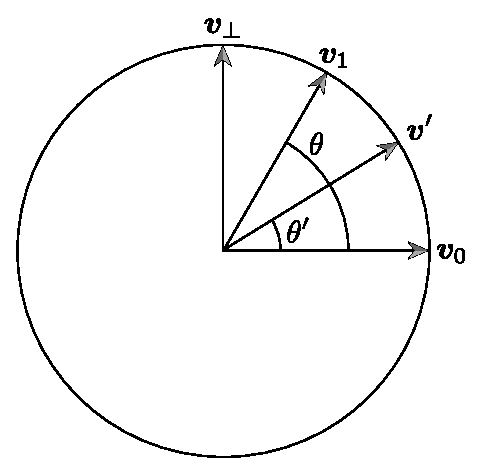
\includegraphics[scale=0.6]{chap02/Quaternionrotation.eps}
    \caption{为了理解四元数球面线性插值,考虑2D下的两个单位圆上的向量$\bm v_0$和$\bm v_1$,
        两者夹角$\theta$。我们想要计算两者间角度为$\theta'$的插值向量。
        为此,我们可以寻找正交于$\bm v_0$的向量$\bm v_{\perp}$,
        再应用三角恒等式$\bm v'=\bm v_0\cos\theta'+\bm v_{\perp}\sin\theta'$。}
    \label{fig:2.17}
\end{figure}

一个计算$\bm q'$的简单方法是先在四元数空间中计算一个正交坐标系统,
一个轴为$\bm q_1$,另一个是与$\bm q_1$正交的四元数,
这样两轴就构成张开$\bm q_1$和$\bm q_2$的基。

有了这个坐标系统,我们就能计算关于$\bm q_1$的旋转
(见\reffig{2.17}展示的2D设置下的概念)。
正交向量$\bm q_{\perp}$可以通过将$\bm q_2$投影到$\bm q_1$并
从$\bm q_2$减去该正交投影得到;
剩余部分保证与$\bm q_1$正交:
\begin{align}\label{eq:2.7}
    \bm q_{\perp}=\bm q_2-(\bm q_1\cdot\bm q_2)\bm q_1\, .
\end{align}
给定坐标系统和规范化的$\bm q_{\perp}$,沿动画路径的四元数为
\begin{align}\label{eq:2.8}
    \bm q'=\bm q_1\cos(\theta t)+\hat{\bm q}_{\perp}\sin(\theta t)\, .
\end{align}

函数\refvar{Slerp}{()}的实现检查看两个四元数是否几乎平行,
是的话它就按顺序对四元数分量用普通的线性插值以避免数值不稳定。
否则,它就用\refeq{2.7}计算正交四元数{\ttfamily qperp},
然后按\refeq{2.8}计算插值的四元数。
\begin{lstlisting}
`\initcode{Quaternion Method Definitions}{=}`
`\refvar{Quaternion}{}` `\initvar{Slerp}{}`( `\refvar{Float}{}` t, const `\refvar{Quaternion}{}` &q1,
                 const `\refvar{Quaternion}{}` &q2) {
     `\refvar{Float}{}` cosTheta = `\refvar[Quaternion::Dot]{Dot}{}`(q1, q2);
    if (cosTheta > .9995f)
        return `\refvar[Quaternion::Normalize]{Normalize}{}`((1 - t) * q1 + t * q2);
    else {
        `\refvar{Float}{}` theta = std::acos(`\refvar{Clamp}{}`(cosTheta, -1, 1));
        `\refvar{Float}{}` thetap = theta * t;
        `\refvar{Quaternion}{}` qperp = `\refvar[Quaternion::Normalize]{Normalize}{}`(q2 - q1 * cosTheta);
        return q1 * std::cos(thetap) + qperp * std::sin(thetap);
    }
}
\end{lstlisting}

\subsection{动画变换实现}\label{sub:动画变换实现}
有了四元数基础知识,我们现在就能实现类\refvar{AnimatedTransform}{}了,
它在pbrt中实现关键帧变换的插值。
其构造函数接收两个变换以及关联的时间值。

正如之前提到的,\refvar{AnimatedTransform}{}将
给定的合成变换矩阵分解为缩放、旋转和平移分量。
分解由方法\refvar[Decompose]{AnimatedTransform::Decompose}{()}执行。

\begin{lstlisting}
`\initcode{AnimatedTransform Method Definitions}{=}\initnext{AnimatedTransformMethodDefinitions}`
`\initvar{AnimatedTransform}{}`::`\refvar{AnimatedTransform}{}`(const `\refvar{Transform}{}` *startTransform,
        `\refvar{Float}{}` startTime, const `\refvar{Transform}{}` *endTransform, `\refvar{Float}{}` endTime)
    : `\refvar{startTransform}{}`(startTransform), `\refvar{endTransform}{}`(endTransform),
      `\refvar{startTime}{}`(startTime), `\refvar{endTime}{}`(endTime),
      `\refvar{actuallyAnimated}{}`(*startTransform != *endTransform) {
    `\refvar{Decompose}{}`(startTransform->m, &`\refvar[AnimatedTransform::T]{T}{}`[0], &`\refvar[AnimatedTransform::R]{R}{}`[0], &`\refvar[AnimatedTransform::S]{S}{}`[0]);
    `\refvar{Decompose}{}`(endTransform->m, &`\refvar[AnimatedTransform::T]{T}{}`[1], &`\refvar[AnimatedTransform::R]{R}{}`[1], &`\refvar[AnimatedTransform::S]{S}{}`[1]);
    `\refcode{Flip R[1] if needed to select shortest path}{}`
    `\refvar{hasRotation}{}` = `\refvar[Quaternion::Dot]{Dot}{}`(`\refvar[AnimatedTransform::R]{R}{}`[0], `\refvar[AnimatedTransform::R]{R}{}`[1]) < 0.9995f;
    `\refcode{Compute terms of motion derivative function}{}`
}
\end{lstlisting}

\begin{lstlisting}
`\initcode{AnimatedTransform Private Data}{=}\initnext{AnimatedTransformPrivateData}`
const `\refvar{Transform}{}` *`\initvar{startTransform}{}`, *`\initvar{endTransform}{}`;
const `\refvar{Float}{}` `\initvar{startTime}{}`, `\initvar{endTime}{}`;
const bool `\initvar{actuallyAnimated}{}`;
`\refvar{Vector3f}{}` `\initvar[AnimatedTransform::T]{T}{}`[2];
`\refvar{Quaternion}{}` `\initvar[AnimatedTransform::R]{R}{}`[2];
`\refvar{Matrix4x4}{}` `\initvar[AnimatedTransform::S]{S}{}`[2];
bool `\initvar{hasRotation}{}`;
\end{lstlisting}

给定一变换的合成矩阵,关于合成它的任何单个变换的信息已经损失了。
例如,给定一先平移在缩放的矩阵乘积,
一个等价矩阵也可以是先缩放再平移(但量不同)。
因此,我们需要为分解选择一个标准变换序列。
此处根据我们的需要,具体选哪个并不重要
(例如在动画系统中这会更重要因为它要分解合成矩阵使其可编辑改变独立分量)。

我们这里只处理\keyindex{仿射变换}{affine transformation}{transformation变换},
渲染系统中的动画相机和几何图元都需要它;
透视变换一般与这样的物体动画无关。

我们将使用下列变换分解:
\begin{align}\label{eq:2.9}
    \bm M=\bm T\bm R\bm S\, ,
\end{align}
其中$\bm M$是给定变换,$\bm T$是平移,$\bm R$是旋转,$\bm S$是缩放。
$\bm S$实际上是一种表示在\emph{某些}坐标系统下的通用缩放
(Shoemake和Duff称之为拉伸\sidenote{译者注:原文stretch。}),
而不一定在是当前坐标系下。
不论哪种情况,它都仍然可以按分量正确地线性插值。
给定\refvar{Matrix4x4}{},方法\refvar{Decompose}{()}计算其分解。
\begin{lstlisting}
`\refcode{AnimatedTransform Method Definitions}{+=}\lastnext{AnimatedTransformMethodDefinitions}`
void `\refvar{AnimatedTransform}{}`::`\initvar{Decompose}{}`(const `\refvar{Matrix4x4}{}` &m, `\refvar{Vector3f}{}` *T,
        `\refvar{Quaternion}{}` *Rquat, `\refvar{Matrix4x4}{}` *S) {
    `\refcode{Extract translation T from transformation matrix}{}`
    `\refcode{Compute new transformation matrix M without translation}{}`
    `\refcode{Extract rotation R from transformation matrix}{}`
    `\refcode{Compute scale S using rotation and original matrix}{}`
}
\end{lstlisting}

提取平移$\bm T$很简单;
可直接从变换矩阵适当的$1\times4$元素中找到它。
\begin{lstlisting}
`\initcode{Extract translation T from transformation matrix}{=}`
T->x = m.`\refvar[Matrix4x4::m]{m}{}`[0][3];
T->y = m.`\refvar[Matrix4x4::m]{m}{}`[1][3];
T->z = m.`\refvar[Matrix4x4::m]{m}{}`[2][3];
\end{lstlisting}

既然我们假设是仿射变换(没有透视分量),
我们可以去掉平移,剩下上面表示缩放和旋转的$3\times3$矩阵。
该矩阵被复制到新矩阵{\ttfamily M}中做进一步处理。
\begin{lstlisting}
`\initcode{Compute new transformation matrix M without translation}{=}`
`\refvar{Matrix4x4}{}` M = m;
for (int i = 0; i < 3; ++i)
    M.`\refvar[Matrix4x4::m]{m}{}`[i][3] = M.`\refvar[Matrix4x4::m]{m}{}`[3][i] = 0.f;
M.`\refvar[Matrix4x4::m]{m}{}`[3][3] = 1.f;
\end{lstlisting}

接着我们想提取纯旋转分量$\bm R$。
我们使用称为\keyindex{极分解}{polar decomposition}{}的技术来完成它。
可以证明矩阵$\bm M$极分解为旋转$\bm R$和缩放$\bm S$可以通过
依次平均$\bm M$和它的逆转置算得
\begin{align}\label{eq:2.10}
    \bm M_{i+1}=\frac{1}{2}(\bm M_i+(\bm M_i^\mathrm{T})^{-1})\, ,
\end{align}
直到收敛于点$\bm M_i=\bm R$。
(容易看到如果$\bm M$是纯旋转,则平均它及其逆转置会保持不变,
因为它的逆等于转置。“扩展阅读”一节有更多讨论
为什么该序列收敛于原始变换旋转分量的参考文献。)
Shoemake和Duff\parencite*{10.5555/155294.155324}证明
结果矩阵是最接近$\bm M$的正交矩阵——我们期望的性质。

为了计算该序列,我们迭代应用\refeq{2.10}直到相邻两项之间的差很小或
执行了固定数目的循环。
实际上,该序列一般收敛得很快。
\begin{lstlisting}
`\initcode{Extract rotation R from transformation matrix}{=}`
`\refvar{Float}{}` norm;
int count = 0;
`\refvar{Matrix4x4}{}` R = M;
do {
    `\refcode{Compute next matrix Rnext in series}{}`
    `\refcode{Compute norm of difference between R and Rnext}{}`
    R = Rnext;
} while (++count < 100 && norm > .0001);
*Rquat = `\refvar{Quaternion}{}`(R);
\end{lstlisting}
\begin{lstlisting}
`\initcode{Compute next matrix Rnext in series}{=}`
`\refvar{Matrix4x4}{}` Rnext;
`\refvar{Matrix4x4}{}` Rit = `\refvar[Matrix4x4::Inverse]{Inverse}{}`(`\refvar[Matrix4x4::Transpose]{Transpose}{}`(R));
for (int i = 0; i < 4; ++i)
    for (int j = 0; j < 4; ++j)
        Rnext.`\refvar[Matrix4x4::m]{m}{}`[i][j] = 0.5f * (R.`\refvar[Matrix4x4::m]{m}{}`[i][j] + Rit.`\refvar[Matrix4x4::m]{m}{}`[i][j]);
\end{lstlisting}
\begin{lstlisting}
`\initcode{Compute norm of difference between R and Rnext}{=}`
norm = 0;
for (int i = 0; i < 3; ++i) {
    `\refvar{Float}{}` n = std::abs(R.`\refvar[Matrix4x4::m]{m}{}`[i][0] - Rnext.`\refvar[Matrix4x4::m]{m}{}`[i][0]) + 
              std::abs(R.`\refvar[Matrix4x4::m]{m}{}`[i][1] - Rnext.`\refvar[Matrix4x4::m]{m}{}`[i][1]) + 
              std::abs(R.`\refvar[Matrix4x4::m]{m}{}`[i][2] - Rnext.`\refvar[Matrix4x4::m]{m}{}`[i][2]);
    norm = std::max(norm, n);
}
\end{lstlisting}

一旦我们从$\bm M$提取了旋转,剩下的全部就是缩放了。
我们想寻找满足$\bm M=\bm R\bm S$的矩阵$\bm S$。
现在我们知道了$\bm R$和$\bm M$,只需解得$\bm S=\bm R^{-1}\bm M$。
\begin{lstlisting}
`\initcode{Compute scale S using rotation and original matrix}{=}`
*S = `\refvar{Matrix4x4::Mul}{}`(`\refvar[Matrix4x4::Inverse]{Inverse}{}`(R), M);
\end{lstlisting}

对于每个旋转矩阵,有两个单位四元数与其矩阵对应且只相差一个符号。
如果我们提取到的两个旋转的点积是负数,则两者之间的slerp不会
在相应的两个旋转之间走最短路径。
令其中一个取负(这里即任意选择第二个)可以改为取到最短路径。
\begin{lstlisting}
`\initcode{Flip R[1] if needed to select shortest path}{=}`
if (`\refvar{Dot}{}`(`\refvar[AnimatedTransform::R]{R}{}`[0], `\refvar[AnimatedTransform::R]{R}{}`[1]) < 0)
    `\refvar[AnimatedTransform::R]{R}{}`[1] = -`\refvar[AnimatedTransform::R]{R}{}`[1];
\end{lstlisting}

方法\refvar{Interpolate}{()}计算给定时刻的插值变换矩阵。
通过插值之前提取的平移、旋转和缩放再相乘得到
表示三种变换综合效应的合成矩阵。
\begin{lstlisting}
`\refcode{AnimatedTransform Method Definitions}{+=}\lastnext{AnimatedTransformMethodDefinitions}`
void `\refvar{AnimatedTransform}{}`::`\initvar{Interpolate}{}`(`\refvar{Float}{}` time, `\refvar{Transform}{}` *t) const {
    `\refcode{Handle boundary conditions for matrix interpolation}{}`
    `\refvar{Float}{}` dt = (time - `\refvar{startTime}{}`) / (`\refvar{endTime}{}` - `\refvar{startTime}{}`);
    `\refcode{Interpolate translation at dt}{}`
    `\refcode{Interpolate rotation at dt}{}`
    `\refcode{Interpolate scale at dt}{}`
    `\refcode{Compute interpolated matrix as product of interpolated components}{}`
}
\end{lstlisting}

如果给定时间值超出存于\refvar{AnimatedTransform}{}的两个变换的时间范围,
则视情况返回开始或结束时刻的变换。
\refvar{AnimatedTransform}{}构造函数也检查两个\refvar{Transform}{}是否相同;
如果是,则没有必要插值。
pbrt中所有支持动画的类都永远为其变换保存了\refvar{AnimatedTransform}{},
而不是视情况保存\refvar{Transform}{}或
\refvar{AnimatedTransform}{}。
尽管确实值得检查这种情况而不必要在两个相等的变换之间插值,
但这简化了它们的实现。
\begin{lstlisting}
`\initcode{Handle boundary conditions for matrix interpolation}{=}`
if (!`\refvar{actuallyAnimated}{}` || time <= `\refvar{startTime}{}`) { 
    *t = *`\refvar{startTransform}{}`;
    return; 
}
if (time >= `\refvar{endTime}{}`) { 
    *t = *`\refvar{endTransform}{}`;
    return; 
}
\end{lstlisting}

变量{\ttfamily dt}保存了从\refvar{startTime}{}到\refvar{endTime}{}范围的偏移量;
在\refvar{startTime}{}处取零,\refvar{endTime}{}处取一。
给定{\ttfamily dt},平移的插值很简单。
\begin{lstlisting}
`\initcode{Interpolate translation at dt}{=}`
`\refvar{Vector3f}{}` trans = (1 - dt) * `\refvar[AnimatedTransform::T]{T}{}`[0] + dt * `\refvar[AnimatedTransform::T]{T}{}`[1];
\end{lstlisting}

开始和结束之间的旋转插值用\refvar{Slerp}{()}例程(\refsub{四元数插值})。
\begin{lstlisting}
`\initcode{Interpolate rotation at dt}{=}`
`\refvar{Quaternion}{}` rotate = `\refvar{Slerp}{}`(dt, `\refvar[AnimatedTransform::R]{R}{}`[0], `\refvar[AnimatedTransform::R]{R}{}`[1]);
\end{lstlisting}

最后,缩放插值矩阵通过对开始和结束缩放矩阵的独立分量插值算得。
因为\refvar{Matrix4x4}{}构造函数把矩阵设置为单位矩阵,
我们不需要初始化{\ttfamily scale}的其他任何元素。
\begin{lstlisting}
`\initcode{Interpolate scale at dt}{=}`
`\refvar{Matrix4x4}{}` scale;
for (int i = 0; i < 3; ++i)
    for (int j = 0; j < 3; ++j)
        scale.m[i][j] = `\refvar{Lerp}{}`(dt, `\refvar[AnimatedTransform::S]{S}{}`[0].m[i][j], `\refvar[AnimatedTransform::S]{S}{}`[1].m[i][j]);
\end{lstlisting}

有了三个插值部分,它们三个变换矩阵的积就给出了最后的结果。
\begin{lstlisting}
`\initcode{Compute interpolated matrix as product of interpolated components}{=}`
*t = `\refvar{Translate}{}`(trans) * rotate.`\refvar{ToTransform}{}`() * `\refvar{Transform}{}`(scale);
\end{lstlisting}

\refvar{AnimatedTransform}{}也使用\refvar{Point3f}{}和
\refvar{Vector3f}{}的时间以及\refvar{Ray}{}的
\refvar{Ray::time}{}
来提供大量直接应用插值变换的方法。
当实际上没有动画时,这些方法比调用\refvar[Interpolate]{AnimatedTransform::Interpolate}{()}再
使用返回的矩阵更高效,因为那种情况下不需要复制变换矩阵。
\begin{lstlisting}
`\initcode{AnimatedTransform Public Methods}{=}`
`\refvar{Ray}{}` operator()(const `\refvar{Ray}{}` &r) const;
`\refvar{RayDifferential}{}` operator()(const `\refvar{RayDifferential}{}` &r) const;
`\refvar{Point3f}{}` operator()(`\refvar{Float}{}` time, const `\refvar{Point3f}{}` &p) const;
`\refvar{Vector3f}{}` operator()(`\refvar{Float}{}` time, const `\refvar{Vector3f}{}` &v) const;
\end{lstlisting}

\subsection{定界移动边界框}\label{sub:定界移动边界框}
给定经过动画变换的\refvar{Bounds3f}{},


\section{交互作用}\label{sec:交互作用}

本章最后的抽象\refvar{SurfaceInteraction}{},表示在2D曲面上某点的局部信息。
例如,第\refchap{形状}的光线-形状相交例程在\refvar{SurfaceInteraction}{}里
返回在交点处的局部微分几何相关信息。
之后,第\refchap{纹理}的纹理代码计算\refvar{SurfaceInteraction}{}表示的曲面上给定点的材料属性。
紧密相关的类\refvar{MediumInteraction}{}用于表示在烟或云等介质中发生光散射的点;
在介绍了额外的预备知识后,它将在\refsec{介质}中定义。
这些类的实现在文件\href{https://github.com/mmp/pbrt-v3/tree/master/src/core/interaction.h}{\ttfamily core/interaction.h}和
\href{https://github.com/mmp/pbrt-v3/tree/master/src/core/interaction.cpp}{\ttfamily core/interaction.cpp}中。

\refvar{SurfaceInteraction}{}和\refvar{MediumInteraction}{}都继承自
一般类\refvar{Interaction}{},它提供了一些常见的成员变量和方法。
系统的一些部分(特别是光源实现)对\refvar{Interaction}{}进行操作,
而曲面和介质相互作用的区别对其并不重要。

\begin{lstlisting}
`\initcode{Interaction Declarations}{=}\initnext{InteractionDeclarations}`
struct `\initvar{Interaction}{}` {
    `\refcode{Interaction Public Methods}{}`
    `\refcode{Interaction Public Data}{}`
};
\end{lstlisting}

有许多\refvar{Interaction}{}构造函数可用;
根据要构造的交互作用类型以及哪种类型的信息相关,接收相应参数集。
以下是其中最一般的一个。
\begin{lstlisting}
`\initcode{Interaction Public Methods}{=}\initnext{InteractionPublicMethods}`
`\refvar{Interaction}{}`(const `\refvar{Point3f}{}` &p, const `\refvar{Normal3f}{}` &n, const `\refvar{Vector3f}{}` &pError,
        const `\refvar{Vector3f}{}` &wo, `\refvar{Float}{}` time,
        const `\refvar{MediumInterface}{}` &mediumInterface)
    : `\refvar[Interaction::p]{p}{}`(p), `\refvar[Interaction::time]{time}{}`(time), `\refvar{pError}{}`(pError), `\refvar[Interaction::wo]{wo}{}`(wo), `\refvar[Interaction::n]{n}{}`(n),
      `\refvar{mediumInterface}{}`(mediumInterface) { }
\end{lstlisting}

所有交互作用必须有关联的点$\bm p$和时间。
\begin{lstlisting}
`\initcode{Interaction Public Data}{=}\initnext{InteractionPublicData}`
`\refvar{Point3f}{}` `\initvar[Interaction::p]{p}{}`;
`\refvar{Float}{}` `\initvar[Interaction::time]{time}{}`;
\end{lstlisting}

对于由光线相交计算的点$\bm p$处的交互作用,
\refvar[Interaction::p]{p}{}值中通常会出现浮点误差。
\refvar{pError}{}给出了该误差的保守边界;
对于介质中的点它取$(0,0,0)$。
关于pbrt控制舍入误差的方法见\refsec{控制舍入误差}{},
关于怎样为不同形状计算该边界见\refsub{定界交点误差}。
\begin{lstlisting}
`\refcode{Interaction Public Data}{+=}\lastnext{InteractionPublicData}`
`\refvar{Vector3f}{}` `\initvar{pError}{}`;
\end{lstlisting}

对于沿光线(要么来自光线-形状相交要么来自在介质中传播的光线)的交互作用,
负的光线方向保存于\refvar[Interaction::wo]{wo}{},
对应于$\bm \omega_{\mathrm{o}}$,
即我们计算一点光量时用来表示出射方向的记号。
对于没有用到出射方向记号的其他类型的交互作用点
(例如形状曲面上由随机采样点求得的),
\refvar[Interaction::wo]{wo}{}的值为$(0,0,0)$。
\begin{lstlisting}
`\refcode{Interaction Public Data}{+=}\lastnext{InteractionPublicData}`
`\refvar{Vector3f}{}` `\initvar[Interaction::wo]{wo}{}`;
\end{lstlisting}

对于曲面上的交互作用,\refvar[Interaction::n]{n}{}保存了该点处的曲面法线。
\begin{lstlisting}
`\refcode{Interaction Public Data}{+=}\lastnext{InteractionPublicData}`
`\refvar{Normal3f}{}` `\initvar[Interaction::n]{n}{}`;
\end{lstlisting}
\begin{lstlisting}
`\refcode{Interaction Public Methods}{+=}\lastnext{InteractionPublicMethods}`
bool `\initvar{IsSurfaceInteraction}{}`() const {
    return `\refvar[Interaction::n]{n}{}` != `\refvar{Normal3f}{}`();
}
\end{lstlisting}

交互作用也需要记录这些点处的散射介质(如果有的话);
这由\refsub{介质交互}定义的类
\refvar{MediumInterface}{}的实例负责处理。
\begin{lstlisting}
`\refcode{Interaction Public Data}{+=}\lastcode{InteractionPublicData}`
`\refvar{MediumInterface}{}` `\initvar{mediumInterface}{}`;
\end{lstlisting}

\subsection{表面交互}\label{sub:表面交互}
\refvar{SurfaceInteraction}{}表示曲面上特定点
(通常是光线与曲面相交求得的位置)的几何信息。
有了这个抽象后处理曲面上点的大部分系统就不用考虑该点所在几何形状的特定类型;
抽象\refvar{SurfaceInteraction}{}提供了关于曲面点的充足信息
以允许一般化实现pbrt剩余部分的着色和几何操作。
\begin{lstlisting}
`\initcode{SurfaceInteraction Declarations}{=}`
class `\initvar{SurfaceInteraction}{}` : public `\refvar{Interaction}{}` {
public:
    `\refcode{SurfaceInteraction Public Methods}{}`
    `\refcode{SurfaceInteraction Public Data}{}`
};
\end{lstlisting}
\begin{lstlisting}
`\initcode{SurfaceInteraction Public Methods}{=}`
`\refvar{SurfaceInteraction}{}`() { }
`\refvar{SurfaceInteraction}{}`(const `\refvar{Point3f}{}` &p, const `\refvar{Vector3f}{}` &pError,const `\refvar{Point2f}{}` &uv,
    const `\refvar{Vector3f}{}` &wo, const `\refvar{Vector3f}{}` &dpdu, const `\refvar{Vector3f}{}` &dpdv,
    const `\refvar{Normal3f}{}` &dndu, const `\refvar{Normal3f}{}` &dndv,
    `\refvar{Float}{}` time, const `\refvar{Shape}{}` *sh);
void `\refvar{SetShadingGeometry}{}`(const `\refvar{Vector3f}{}` &dpdu, const `\refvar{Vector3f}{}` &dpdv,
     const `\refvar{Normal3f}{}` &dndu, const `\refvar{Normal3f}{}` &dndv, bool orientationIsAuthoritative);
void `\initvar{ComputeScatteringFunctions}{}`(const `\refvar{RayDifferential}{}` &ray,
    `\refvar{MemoryArena}{}` &arena, bool allowMultipleLobes = false,
    `\refvar{TransportMode}{}` mode = `\refvar{TransportMode}{}`::`\refvar{Radiance}{}`);
void `\initvar{ComputeDifferentials}{}`(const `\refvar{RayDifferential}{}` &r) const;
`\refvar{Spectrum}{}` `\initvar[SurfaceInteraction::Le]{Le}{}`(const `\refvar{Vector3f}{}` &w) const;
\end{lstlisting}

除了来自基类\refvar{Interaction}{}的点\refvar[Interaction::p]{p}{}和
曲面法线\refvar[Interaction::n]{n}{},
\refvar{SurfaceInteraction}{}还存储了来自曲面参数化的坐标$(u,v)$以及
该点的参数化偏导数$\displaystyle\frac{\partial \bm p}{\partial u}$
和$\displaystyle\frac{\partial \bm p}{\partial v}$。
这些值的描述见\reffig{2.19}。
保有指向该点所在\refvar{Shape}{}(下章将介绍类\refvar{Shape}{})的指针
以及曲面法线的偏导数也很有用。
\begin{lstlisting}
`\initcode{SurfaceInteraction Public Data}{=}\initnext{SurfaceInteractionPublicData}`
`\refvar{Point2f}{}` `\initvar[SurfaceInteraction::uv]{uv}{}`;
`\refvar{Vector3f}{}` `\initvar[SurfaceInteraction::dpdu]{dpdu}{}`, `\initvar[SurfaceInteraction::dpdv]{dpdv}{}`;
`\refvar{Normal3f}{}` `\initvar[SurfaceInteraction::dndu]{dndu}{}`, `\initvar[SurfaceInteraction::dndv]{dndv}{}`;
const `\refvar{Shape}{}` *`\initvar{shape}{}` = nullptr;
\end{lstlisting}

\begin{figure}[htbp]
    \centering%LaTeX with PSTricks extensions
%%Creator: Inkscape 1.0.1 (3bc2e813f5, 2020-09-07)
%%Please note this file requires PSTricks extensions
\psset{xunit=.5pt,yunit=.5pt,runit=.5pt}
\begin{pspicture}(179.24000549,190.82000732)
{
\newrgbcolor{curcolor}{0 0 0}
\pscustom[linewidth=1,linecolor=curcolor]
{
\newpath
\moveto(151.91,155.49000732)
\curveto(151.91,155.49000732)(140.58,133.65000732)(107.56,136.66000732)
\curveto(74.54,139.67000732)(58.56,162.51000732)(25.73,135.85000732)
\curveto(6.22,120.00000732)(4.94,107.63000732)(0.47,95.05000732)
}
}
{
\newrgbcolor{curcolor}{0 0 0}
\pscustom[linewidth=1,linecolor=curcolor]
{
\newpath
\moveto(178.75999451,59.71000671)
\lineto(151.86999512,155.93000793)
}
}
{
\newrgbcolor{curcolor}{0 0 0}
\pscustom[linewidth=1,linecolor=curcolor]
{
\newpath
\moveto(27.26000023,0.63000488)
\lineto(0.54000002,95.49000549)
}
}
{
\newrgbcolor{curcolor}{0 0 0}
\pscustom[linewidth=1,linecolor=curcolor]
{
\newpath
\moveto(178.74,60.23000732)
\curveto(178.74,60.23000732)(167.14,38.01000732)(134.12,41.02000732)
\curveto(101.1,44.03000732)(85.12,66.86000732)(52.29,40.21000732)
\curveto(33.35,24.82000732)(31.47,12.37000732)(27.29,0.21000732)
}
}
{
\newrgbcolor{curcolor}{0 0 0}
\pscustom[linewidth=0.5,linecolor=curcolor]
{
\newpath
\moveto(118.28,89.89000732)
\lineto(55.03,89.21000732)
\lineto(40.66,118.93000732)
\lineto(103.92,119.61000732)
\closepath
}
}
{
\newrgbcolor{curcolor}{0 0 0}
\pscustom[linewidth=1,linecolor=curcolor]
{
\newpath
\moveto(79.68000031,103.34000397)
\lineto(79.68000031,164.19000816)
}
}
{
\newrgbcolor{curcolor}{0 0 0}
\pscustom[linestyle=none,fillstyle=solid,fillcolor=curcolor]
{
\newpath
\moveto(85.19,159.28000732)
\lineto(79.68,163.54000732)
\lineto(74.18,159.28000732)
\lineto(79.68,172.29000732)
\closepath
}
}
{
\newrgbcolor{curcolor}{0.65098041 0.65098041 0.65098041}
\pscustom[linestyle=none,fillstyle=solid,fillcolor=curcolor]
{
\newpath
\moveto(83.99,160.84000732)
\lineto(79.68,170.98000732)
\lineto(79.68,164.17000732)
\closepath
}
}
{
\newrgbcolor{curcolor}{0.40000001 0.40000001 0.40000001}
\pscustom[linestyle=none,fillstyle=solid,fillcolor=curcolor]
{
\newpath
\moveto(75.39,160.84000732)
\lineto(79.68,170.98000732)
\lineto(79.68,164.17000732)
\closepath
}
}
{
\newrgbcolor{curcolor}{0 0 0}
\pscustom[linestyle=none,fillstyle=solid,fillcolor=curcolor]
{
\newpath
\moveto(83.07000375,103.88000488)
\curveto(83.07000375,106.91820179)(79.39696119,108.4391858)(77.24889196,106.29111658)
\curveto(75.10082274,104.14304736)(76.62180676,100.4700048)(79.66000366,100.4700048)
\curveto(82.69820057,100.4700048)(84.21918458,104.14304736)(82.07111536,106.29111658)
\curveto(79.92304614,108.4391858)(76.25000358,106.91820179)(76.25000358,103.88000488)
\curveto(76.25000358,100.84180798)(79.92304614,99.32082396)(82.07111536,101.46889319)
\curveto(84.21918458,103.61696241)(82.69820057,107.29000497)(79.66000366,107.29000497)
\curveto(76.62180676,107.29000497)(75.10082274,103.61696241)(77.24889196,101.46889319)
\curveto(79.39696119,99.32082396)(83.07000375,100.84180798)(83.07000375,103.88000488)
\closepath
}
}
{
\newrgbcolor{curcolor}{0 0 0}
\pscustom[linewidth=1,linecolor=curcolor]
{
\newpath
\moveto(79.51000214,103.76000977)
\lineto(108.83999634,71.65000916)
}
}
{
\newrgbcolor{curcolor}{0 0 0}
\pscustom[linestyle=none,fillstyle=solid,fillcolor=curcolor]
{
\newpath
\moveto(101.46,71.57000732)
\lineto(108.4,72.13000732)
\lineto(109.59,78.99000732)
\lineto(114.3,65.67000732)
\closepath
}
}
{
\newrgbcolor{curcolor}{0.65098041 0.65098041 0.65098041}
\pscustom[linestyle=none,fillstyle=solid,fillcolor=curcolor]
{
\newpath
\moveto(103.4,71.23000732)
\lineto(113.42,66.64000732)
\lineto(108.82,71.67000732)
\closepath
}
}
{
\newrgbcolor{curcolor}{0.40000001 0.40000001 0.40000001}
\pscustom[linestyle=none,fillstyle=solid,fillcolor=curcolor]
{
\newpath
\moveto(109.75,77.03000732)
\lineto(113.42,66.64000732)
\lineto(108.82,71.67000732)
\closepath
}
}
{
\newrgbcolor{curcolor}{0 0 0}
\pscustom[linewidth=1,linecolor=curcolor]
{
\newpath
\moveto(122.47000122,99.83000946)
\lineto(79.51000214,103.96000671)
}
}
{
\newrgbcolor{curcolor}{0 0 0}
\pscustom[linestyle=none,fillstyle=solid,fillcolor=curcolor]
{
\newpath
\moveto(118.11,105.77000732)
\lineto(121.82,99.89000732)
\lineto(117.05,94.82000732)
\lineto(130.53,99.05000732)
\closepath
}
}
{
\newrgbcolor{curcolor}{0.65098041 0.65098041 0.65098041}
\pscustom[linestyle=none,fillstyle=solid,fillcolor=curcolor]
{
\newpath
\moveto(119.54,104.43000732)
\lineto(129.23,99.18000732)
\lineto(122.45,99.83000732)
\closepath
}
}
{
\newrgbcolor{curcolor}{0.40000001 0.40000001 0.40000001}
\pscustom[linestyle=none,fillstyle=solid,fillcolor=curcolor]
{
\newpath
\moveto(118.72,95.87000732)
\lineto(129.23,99.18000732)
\lineto(122.45,99.83000732)
\closepath
}
}
{
\newrgbcolor{curcolor}{0 0 0}
\pscustom[linestyle=none,fillstyle=solid,fillcolor=curcolor]
{
\newpath
\moveto(59.57826732,97.90235348)
\curveto(59.50326732,97.56485348)(59.46576732,97.52735348)(59.42826732,97.48985348)
\curveto(59.31576732,97.45235348)(59.05326732,97.45235348)(58.82826732,97.45235348)
\curveto(58.41576732,97.45235348)(57.96576732,97.45235348)(57.96576732,96.77735348)
\curveto(57.96576732,96.51485348)(58.19076732,96.32735348)(58.45326732,96.32735348)
\curveto(59.12826732,96.32735348)(59.91576732,96.40235348)(60.62826732,96.40235348)
\curveto(61.49076732,96.40235348)(62.39076732,96.32735348)(63.21576732,96.32735348)
\curveto(63.36576732,96.32735348)(63.81576732,96.32735348)(63.81576732,97.03985348)
\curveto(63.81576732,97.45235348)(63.44076732,97.45235348)(63.21576732,97.45235348)
\curveto(62.87826732,97.45235348)(62.46576732,97.45235348)(62.16576732,97.48985348)
\lineto(63.21576732,101.65235348)
\curveto(63.55326732,101.31485348)(64.34076732,100.78985348)(65.61576732,100.78985348)
\curveto(69.77826732,100.78985348)(72.36576732,104.57735348)(72.36576732,107.83985348)
\curveto(72.36576732,110.80235348)(70.15326732,111.77735348)(68.16576732,111.77735348)
\curveto(66.47826732,111.77735348)(65.24076732,110.83985348)(64.86576732,110.50235348)
\curveto(63.92826732,111.77735348)(62.35326732,111.77735348)(62.09076732,111.77735348)
\curveto(61.22826732,111.77735348)(60.51576732,111.28985348)(60.02826732,110.42735348)
\curveto(59.42826732,109.45235348)(59.09076732,108.17735348)(59.09076732,108.06485348)
\curveto(59.09076732,107.72735348)(59.46576732,107.72735348)(59.69076732,107.72735348)
\curveto(59.95326732,107.72735348)(60.02826732,107.72735348)(60.14076732,107.83985348)
\curveto(60.21576732,107.87735348)(60.21576732,107.95235348)(60.36576732,108.55235348)
\curveto(60.81576732,110.46485348)(61.37826732,110.91485348)(61.97826732,110.91485348)
\curveto(62.24076732,110.91485348)(62.54076732,110.83985348)(62.54076732,110.05235348)
\curveto(62.54076732,109.67735348)(62.46576732,109.33985348)(62.39076732,109.00235348)
\closepath
\moveto(65.09076732,109.37735348)
\curveto(65.76576732,110.20235348)(66.89076732,110.91485348)(68.05326732,110.91485348)
\curveto(69.55326732,110.91485348)(69.66576732,109.63985348)(69.66576732,109.11485348)
\curveto(69.66576732,107.87735348)(68.84076732,104.91485348)(68.46576732,103.97735348)
\curveto(67.71576732,102.25235348)(66.55326732,101.65235348)(65.57826732,101.65235348)
\curveto(64.15326732,101.65235348)(63.59076732,102.77735348)(63.59076732,103.03985348)
\lineto(63.62826732,103.37735348)
\closepath
\moveto(65.09076732,109.37735348)
}
}
{
\newrgbcolor{curcolor}{0 0 0}
\pscustom[linestyle=none,fillstyle=solid,fillcolor=curcolor]
{
\newpath
\moveto(78.04515732,183.11689348)
\curveto(77.70765732,184.31689348)(76.39515732,184.91689348)(75.08265732,184.91689348)
\curveto(74.22015732,184.91689348)(73.54515732,184.42939348)(73.02015732,183.56689348)
\curveto(72.42015732,182.59189348)(72.08265732,181.31689348)(72.08265732,181.20439348)
\curveto(72.08265732,180.86689348)(72.45765732,180.86689348)(72.68265732,180.86689348)
\curveto(72.94515732,180.86689348)(73.02015732,180.86689348)(73.13265732,180.97939348)
\curveto(73.20765732,181.01689348)(73.20765732,181.09189348)(73.35765732,181.69189348)
\curveto(73.80765732,183.52939348)(74.33265732,184.05439348)(74.97015732,184.05439348)
\curveto(75.34515732,184.05439348)(75.53265732,183.82939348)(75.53265732,183.19189348)
\curveto(75.53265732,182.77939348)(75.42015732,182.40439348)(75.19515732,181.42939348)
\curveto(75.00765732,180.75439348)(74.78265732,179.81689348)(74.67015732,179.29189348)
\lineto(73.80765732,175.91689348)
\curveto(73.73265732,175.61689348)(73.62015732,175.12939348)(73.62015732,174.97939348)
\curveto(73.62015732,174.49189348)(73.99515732,173.92939348)(74.74515732,173.92939348)
\curveto(75.98265732,173.92939348)(76.24515732,175.01689348)(76.43265732,175.72939348)
\lineto(77.10765732,178.42939348)
\curveto(77.18265732,178.72939348)(77.78265732,181.20439348)(77.85765732,181.27939348)
\curveto(77.85765732,181.42939348)(78.53265732,182.47939348)(79.32015732,183.15439348)
\curveto(79.99515732,183.67939348)(80.78265732,184.05439348)(81.79515732,184.05439348)
\curveto(82.39515732,184.05439348)(82.99515732,183.82939348)(82.99515732,182.66689348)
\curveto(82.99515732,181.27939348)(81.94515732,178.50439348)(81.49515732,177.30439348)
\curveto(81.19515732,176.66689348)(81.15765732,176.47939348)(81.15765732,176.06689348)
\curveto(81.15765732,174.67939348)(82.54515732,173.92939348)(83.85765732,173.92939348)
\curveto(86.37015732,173.92939348)(87.57015732,177.19189348)(87.57015732,177.64189348)
\curveto(87.57015732,177.97939348)(87.23265732,177.97939348)(87.00765732,177.97939348)
\curveto(86.70765732,177.97939348)(86.55765732,177.97939348)(86.44515732,177.67939348)
\curveto(85.65765732,175.01689348)(84.38265732,174.79189348)(84.00765732,174.79189348)
\curveto(83.82015732,174.79189348)(83.59515732,174.79189348)(83.59515732,175.27939348)
\curveto(83.59515732,175.84189348)(83.82015732,176.44189348)(84.04515732,177.04189348)
\curveto(84.45765732,178.01689348)(85.54515732,180.82939348)(85.54515732,182.14189348)
\curveto(85.54515732,184.35439348)(83.70765732,184.91689348)(81.98265732,184.91689348)
\curveto(81.49515732,184.91689348)(79.73265732,184.91689348)(78.04515732,183.11689348)
\closepath
\moveto(78.04515732,183.11689348)
}
}
\end{pspicture}

    \caption{点$\bm p$附近的局部微分结构。曲面的参数化偏导数$\displaystyle\frac{\partial \bm p}{\partial u}$
        和$\displaystyle\frac{\partial \bm p}{\partial v}$位于切平面内但不必正交。
        曲面法线$\bm n$由$\displaystyle\frac{\partial \bm p}{\partial u}$
        和$\displaystyle\frac{\partial \bm p}{\partial v}$的叉积给出。
        向量$\displaystyle\frac{\partial \bm n}{\partial u}$和
        $\displaystyle\frac{\partial \bm n}{\partial v}$(此处没有画出)
        记录当我们沿曲面移动$u$和$v$时曲面法线的微分变化。}
    \label{fig:2.19}
\end{figure}

该表示隐式地假设了形状有参数化描述——
对于一定范围的$(u,v)$值,曲面上的点由某函数$f$给出即$\bm p=f(u,v)$。
尽管这并不适用于所有形状,
但pbrt支持的所有形状至少都有一个局部参数化描述,
所以既然这在别处(例如第\refchap{纹理}的纹理抗锯齿)很有帮助,
我们就继续使用参数化表示。

\refvar{SurfaceInteraction}{}的构造函数接收所有设置这些值的参数。
它计算偏导数的叉积作为法线。
\begin{lstlisting}
`\initcode{SurfaceInteraction Method Definitions}{=}\initnext{SurfaceInteractionMethodDefinitions}`
`\refvar{SurfaceInteraction}{}`::`\refvar{SurfaceInteraction}{}`(const `\refvar{Point3f}{}` &p,
    const `\refvar{Vector3f}{}` &pError, const `\refvar{Point2f}{}` &uv, const `\refvar{Vector3f}{}` &wo,
    const `\refvar{Vector3f}{}` &dpdu, const `\refvar{Vector3f}{}` &dpdv,
    const `\refvar{Normal3f}{}` &dndu, const `\refvar{Normal3f}{}` &dndv,
    `\refvar{Float}{}` time, const `\refvar{Shape}{}` *shape)
    : `\refvar{Interaction}{}`(p, `\refvar{Normal3f}{}`(`\refvar{Normalize}{}`(`\refvar{Cross}{}`(dpdu, dpdv))), pError, wo,
    time, nullptr),
    `\refvar[SurfaceInteraction::uv]{uv}{}`(uv), `\refvar[SurfaceInteraction::dpdu]{dpdu}{}`(dpdu), `\refvar[SurfaceInteraction::dpdv]{dpdv}{}`(dpdv), `\refvar[SurfaceInteraction::dndu]{dndu}{}`(dndu), `\refvar[SurfaceInteraction::dndv]{dndv}{}`(dndv),
    `\refvar{shape}{}`(shape) {
    `\refcode{Initialize shading geometry from true geometry}{}`
    `\refcode{Adjust normal based on orientation and handedness}{}`
}
\end{lstlisting}

\refvar{SurfaceInteraction}{}存储了曲面法线以及各种偏导数的第二个实例
来表示这些量因为凹凸贴图或用三角形为每个顶点插值法线而可能生成的扰动值。
系统一些部分使用该着色几何体\sidenote{译者注:原文shading geometry。},而其他的则需要处理原始量。
\begin{lstlisting}
`\refcode{SurfaceInteraction Public Data}{+=}\lastnext{SurfaceInteractionPublicData}`
struct {
    `\refvar{Normal3f}{}` `\initvar[shading::n]{n}{}`;
    `\refvar{Vector3f}{}` `\initvar[shading::dpdu]{dpdu}{}`, `\initvar[shading::dpdv]{dpdv}{}`;
    `\refvar{Normal3f}{}` `\initvar[shading::dndu]{dndu}{}`, `\initvar[shading::dndv]{dndv}{}`;
} `\initvar{shading}{}`;
\end{lstlisting}

着色几何值在构造函数中初始化以匹配原始曲面几何体。
如果存在着色几何体,则通常直到\refvar{SurfaceInteraction}{}
构造函数运行一段时间后才计算它。
稍后定义的方法\refvar{SetShadingGeometry}{()}
将更新着色几何体。
\begin{lstlisting}
`\initcode{Initialize shading geometry from true geometry}{=}`
`\refvar{shading}{}`.`\refvar[shading::n]{n}{}` = n;
`\refvar{shading}{}`.`\refvar[shading::dpdu]{dpdu}{}` = dpdu;
`\refvar{shading}{}`.`\refvar[shading::dpdv]{dpdv}{}` = dpdv;
`\refvar{shading}{}`.`\refvar[shading::dndu]{dndu}{}` = dndu;
`\refvar{shading}{}`.`\refvar[shading::dndv]{dndv}{}` = dndv;
\end{lstlisting}

曲面法线对pbrt有特殊意义,
它假设对于闭合形状,法线指向形状外部。
对于用作面光源的几何体,光只从法线指向的那一侧曲面发出;另一侧是黑的。
因为法线有这样的特殊意义,pbrt为用户提供了机制翻转法线的朝向,使其指向相反方向。
pbrt输入文件中的\refvar{reverseOrientation}{}指令将法线翻转为相反的非默认方向。
因此,有必要检查所给的\refvar{Shape}{}是否设置了相应标识,
如果有则在此切换法线方向。

然而还必须考虑另一个影响法线朝向的因素。
如果\refvar{Shape}{}的变换矩阵把物体坐标系的惯用手
从pbrt默认的左手坐标系变为右手,则我们也需切换法线的朝向。
为了理解为何会这样,考虑一个缩放矩阵$\bm S(1,1,-1)$。
我们自然能料到该缩放会改变法线的方向,当然我们也能
通过$\displaystyle\bm n=\frac{\partial\bm p}{\partial u}\times\frac{\partial\bm p}{\partial v}$计算法线
\sidenote{译者注:为了帮助读者理解该式,笔者加上了括号以澄清运算顺序。},
\begin{align*}
    \left(\bm S(1,1,-1)\frac{\partial\bm p}{\partial u}\right)\times\left(\bm S(1,1,-1)\frac{\partial\bm p}{\partial v}\right) & =\bm S(-1,-1,1)\left(\frac{\partial\bm p}{\partial u}\times\frac{\partial\bm p}{\partial v}\right) \\
                                                                                                                               & =\bm S(-1,-1,1)\bm n                                                                               \\
                                                                                                                               & \neq \bm S(1,1,-1)\bm n\, .
\end{align*}
因此,如果变换切换了坐标系的惯用手,则它也需要翻转法线的方向,
因为用叉积计算法线方向不会考虑该翻转。

如果满足了两个条件中的一个而不是两个,则要交换法线方向;
如果都满足,它们的作用会抵消。异或运算测试该条件。
\begin{lstlisting}
`\initcode{Adjust normal based on orientation and handedness}{=}`
if (`\refvar{shape}{}` && (`\refvar{shape}{}`->`\refvar{reverseOrientation}{}` ^
              `\refvar{shape}{}`->`\refvar{transformSwapsHandedness}{}`)) {
    `\refvar[Interaction::n]{n}{}` *= -1;
    `\refvar{shading}{}`.`\refvar[shading::n]{n}{}` *= -1;
}
\end{lstlisting}

计算一个着色坐标系时,\refvar{SurfaceInteraction}{}通过
\refvar{SetShadingGeometry}{()}
方法得到更新。
\begin{lstlisting}
`\refcode{SurfaceInteraction Method Definitions}{+=}\lastnext{SurfaceInteractionMethodDefinitions}`
void `\refvar{SurfaceInteraction}{}`::`\initvar{SetShadingGeometry}{}`(const `\refvar{Vector3f}{}` &dpdus,
        const `\refvar{Vector3f}{}` &dpdvs, const `\refvar{Normal3f}{}` &dndus,
        const `\refvar{Normal3f}{}` &dndvs, bool orientationIsAuthoritative) {
    `\refcode{Compute shading.n for SurfaceInteraction}{}`
    `\refcode{Initialize shading partial derivative values}{}`
}
\end{lstlisting}

在像之前那样执行同样的叉积(可能翻转了法线朝向)计算初始着色法线后,
如果需要的话实现就翻转着色法线或真正的几何法线,
使得两法线位于同一半球。
因为着色法线通常表示几何法线相对小的扰动,它们两个应该总是位于同一半球。
根据上下文,要么是几何法线要么是着色法线可能更权威地指向正确的曲面“外侧”,
所以调用者在需要时传入一个布尔值决定要翻转哪一个。
\begin{lstlisting}
`\initcode{Compute shading.n for SurfaceInteraction}{=}`
`\refvar{shading}{}`.`\refvar[shading::n]{n}{}` = `\refvar{Normalize}{}`((`\refvar{Normal3f}{}`)`\refvar{Cross}{}`(dpdus, dpdvs));
if (`\refvar{shape}{}` && (`\refvar{shape}{}`->`\refvar{reverseOrientation}{}` ^
              `\refvar{shape}{}`->`\refvar{transformSwapsHandedness}{}`))
    `\refvar{shading}{}`.`\refvar[shading::n]{n}{}` = -`\refvar{shading}{}`.`\refvar[shading::n]{n}{}`;
if (orientationIsAuthoritative)
    `\refvar[Interaction::n]{n}{}` = `\refvar{Faceforward}{}`(`\refvar[Interaction::n]{n}{}`, `\refvar{shading}{}`.`\refvar[shading::n]{n}{}`);
else
    `\refvar{shading}{}`.`\refvar[shading::n]{n}{}` = `\refvar{Faceforward}{}`(`\refvar{shading}{}`.`\refvar[shading::n]{n}{}`, `\refvar[Interaction::n]{n}{}`);
\end{lstlisting}
\begin{lstlisting}
`\initcode{Initialize shading partial derivative values}{=}`
`\refvar{shading}{}`.`\refvar[shading::dpdu]{dpdu}{}` = dpdus;
`\refvar{shading}{}`.`\refvar[shading::dpdv]{dpdv}{}` = dpdvs;
`\refvar{shading}{}`.`\refvar[shading::dndu]{dndu}{}` = dndus;
`\refvar{shading}{}`.`\refvar[shading::dndv]{dndv}{}` = dndvs;
\end{lstlisting}

我们将向\refvar{Transform}{}添加一个方法以变换\refvar{SurfaceInteraction}{}。
多数成员按需要要么直接变换要么复制,
但有了pbrt在计算交点时用来定界浮点误差的方法,
对成员变量\refvar[Interaction::p]{p}{}和\refvar{pError}{}的变换需要足够细心。
负责它的代码片\refcode{Transform p and pError in SurfaceInteraction}{}
定义于讨论浮点舍入误差的\refsec{控制舍入误差}。
\begin{lstlisting}
`\refcode{Transform Method Definitions}{+=}\lastnext{TransformMethodDefinitions}`
`\refvar{SurfaceInteraction}{}`
`\refvar{Transform}{}`::operator()(const `\refvar{SurfaceInteraction}{}` &si) const {
    `\refvar{SurfaceInteraction}{}` ret;
    `\refcode{Transform p and pError in SurfaceInteraction}{}`
    `\refcode{Transform remaining members of SurfaceInteraction}{}`
    return ret; 
}
\end{lstlisting}
\begin{lstlisting}
`\initcode{Transform remaining members of SurfaceInteraction}{=}`
const `\refvar{Transform}{}` &t = *this;
ret.n = `\refvar{Normalize}{}`(t(si.n));
ret.wo = t(si.wo);
ret.time = si.time;
ret.mediumInterface = si.mediumInterface;
ret.uv = si.uv;
ret.shape = si.shape;
ret.dpdu = t(si.dpdu);
ret.dpdv = t(si.dpdv);
ret.dndu = t(si.dndu);
ret.dndv = t(si.dndv);
ret.shading.n = `\refvar{Normalize}{}`(t(si.shading.n));
ret.shading.dpdu = t(si.shading.dpdu);
ret.shading.dpdv = t(si.shading.dpdv);
ret.shading.dndu = t(si.shading.dndu);
ret.shading.dndv = t(si.shading.dndv);
ret.dudx = si.dudx;
ret.dvdx = si.dvdx;
ret.dudy = si.dudy;
ret.dvdy = si.dvdy;
ret.dpdx = t(si.dpdx);
ret.dpdy = t(si.dpdy);
ret.bsdf = si.bsdf;
ret.bssrdf = si.bssrdf;
ret.primitive = si.primitive;
//    ret.n = Faceforward(ret.n, ret.shading.n);
ret.shading.n = `\refvar{Faceforward}{}`(ret.shading.n, ret.n);
\end{lstlisting}

\section{扩展阅读}\label{sec:扩展阅读2}
\citeauthor{10.1007/978-3-642-61542-9_19}、\citeauthor{10.1145/282957.282969}
以及他们的合作者主张
\citep{10.1007/978-3-642-61542-9_19,10.1145/282957.282969,Mann97acoordinate}

\section{习题}\label{sec:习题02}

\begin{enumerate}
    \item \circleone 利用问题的对称性寻找一种更高效的方法变换轴对齐的边界框:
          因为八个顶点是三个轴对齐基向量与单个顶点的线性组合,所以可以
          用比我们介绍的高效得多的方法\citep{10.5555/90767.90922}找到它们变换后的边界框。
    \item \circletwo 可以通过使用许多非正交块\sidenote{译者注:原文slab。}的交集计算包围物体的更紧致边界,而不是方框。
          扩展pbrt中的边界框表示以允许用户指定任意块构成的边界。
          \begin{figure}[htb]
              \centering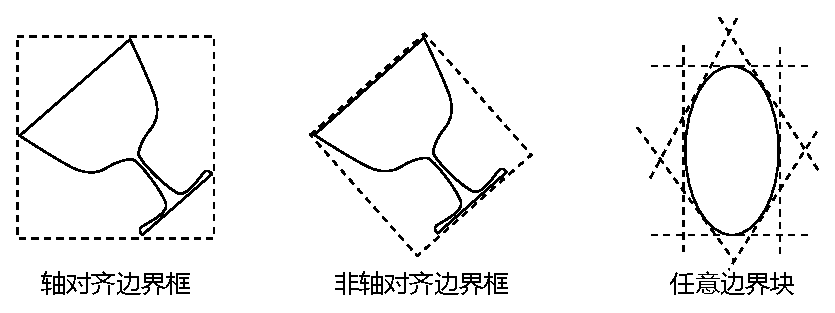
\includegraphics[width=0.8\linewidth]{chap02/Boundingchoices.eps}
          \end{figure}
    \item \circleone 修改pbrt使其像\refvar{Vector3f}{}那样变换\refvar{Normal3f}{},
          并创建因该bug而给出明显错误图像的场景。(完成后别忘了从你的源码拷贝中清除该修改!)
    \item \circletwo 例如,如果一个变换只有平移分量是时变的,则\refvar{AnimatedTransform}{}
          的实现会不必要地计算两个相同旋转之间的插值。修改\refvar{AnimatedTransform}{}
          的实现使其在不需要当前实现中完整一般性的情况下避免这些工作。
          对于适用于你的优化的场景,你观察到了多大的性能变化?
\end{enumerate}

\noindent{\bfseries 第1题解答}\sidenote{译者注:这是笔者根据原文所给参考文献摘录的。}
\begin{algorithm}[htb]
    \SetAlgoNoLine
    \caption{Transform\_Interval\_Box($\bm M,\bm T,\bm A,\bm B$)}
    \KwIn{$3\times3$变换矩阵$\bm M$,平移变换$\bm T$,边界框$\bm A$}
    \KwOut{边界框$\bm B$}
    \For{$i=1\cdots3$}{
    \tcp{从$T_i$处的退化区间开始考虑平移}
    $B_i^{\min}\leftarrow T_i$\;
    $B_i^{\max}\leftarrow T_i$\;
    \tcp{通过计算最小和最大元素与$\bm M$第$i$行的积来求得极值}
    \For{$j=1\cdots3$}{
    $a\leftarrow M_{i,j}*A_j^{\min}$\;
    $b\leftarrow M_{i,j}*A_j^{\max}$\;
    $B_i^{\min}\leftarrow B_i^{\min}+\min(a,b)$\;
    $B_i^{\max}\leftarrow B_i^{\max}+\max(a,b)$\;
    }
    }
\end{algorithm}

{\noindent\hfil$=========$\hfil{\color{red}{施工分割线}}\hfil$=========$\
\input{content/chap02ex01.tex}

\section{译者补充:分解旋转矩阵}\label{sec:译者补充:分解旋转矩阵}
\begin{remark}
    本节内容不是原书内容,而是译者自学补充的,请酌情参考和斧正。
\end{remark}

本节内容主要依据文献\citep{doi:10.1137/0907079,10.5555/155294.155324}整理而成,
给出分解旋转矩阵算法收敛性和最优性的证明。

从只含有旋转$\bm R$和缩放$\bm S$的$3\times3$可逆矩阵$\bm M=\bm R\bm S$中
分解出旋转矩阵,可以利用序列$\displaystyle\{\bm M_i\}_{i=0}^{\infty}$:
\begin{align}
    \bm M_0     & =\bm M\, ,                                                         \\
    \bm M_{i+1} & =\frac{1}{2}(\bm M_i+\bm M_i^{-\mathrm{T}}),\quad i=0,1,\cdots\, ,
\end{align}
此时$\displaystyle \lim\limits_{i \to \infty}{\bm M_i}$必存在
且在Frobenius范数\sidenote{矩阵所有元素的平方和。}度量下最接近$\bm M$,可作为$\bm R$或$-\bm R$,
然后反解$\bm S=\bm R^{-1}\bm M$。

证明该算法之前,先介绍实方阵的正交对角分解定理:
\begin{theorem}
    对于任意可逆方阵$\bm A\in\mathbb{R}^{n\times n}$,
    存在正交矩阵$\bm P$和$\bm Q$以及对角矩阵$\bm \varSigma$,使得
    \begin{align}
        \bm A=\bm P\bm \varSigma\bm Q^{-1}\, ,
    \end{align}
    其中$\bm \varSigma=\mathrm{diag}(\sigma_1,\sigma_2,\cdots,\sigma_n)$,
    $\sigma_k>0$,$k=1,2,\cdots,n$。
\end{theorem}

我们从两方面证明这个算法:
\begin{itemize}
    \item 收敛性:该算法中必存在极限$\displaystyle\lim\limits_{i\rightarrow\infty}\bm M_i$,
          且为正交矩阵。
    \item 最优性:在Frobenius范数度量下$\displaystyle\lim\limits_{i\rightarrow\infty}\bm M_i$
          最接近$\bm M$。
\end{itemize}

\subsection{收敛性}\label{sub:收敛性02ex02}
\begin{prove}
    依据实方阵的正交对角分解定理,存在正交矩阵$\bm P$和$\bm Q$以及对角矩阵$\bm \varSigma$,使得
    \begin{align}\label{eq:02ex.04}
        \bm M=\bm P\bm \varSigma\bm Q^{-1}\, ,
    \end{align}
    其中${\bm \varSigma}=\mathrm{diag}(\sigma_1,\sigma_2,\sigma_3)$,
    $\sigma_k>0$,$k=1,2,3$。

    构造序列$\displaystyle\{\bm M_i\}_{i=0}^{\infty}$:
    \begin{align}
        \bm M_0     & =\bm M\, ,                                                           \\
        \bm M_{i+1} & =\frac{1}{2}(\bm M_i+\bm M_i^{-\mathrm{T}}),\quad i=0,1,2,\cdots\, .
    \end{align}
    再构造另一个序列$\displaystyle\{\bm D_i\}_{i=0}^{\infty}$:
    \begin{align}
        \bm D_i=\bm P^{-1}\bm M_i\bm Q,\quad i=0,1,2,\cdots\, .
    \end{align}
    取$i=0$可得
    \begin{align}
        \bm D_0=\bm \varSigma\, .
    \end{align}
    即$\bm D_0$是对角矩阵且主对角线均为正。

    另一方面,还可得到递推关系
    \begin{align}
        \bm D_{i+1}=\frac{1}{2}(\bm D_i+\bm D_i^{-\mathrm{T}})\, .
    \end{align}
    可以看出如果$\bm D_i$是主对角线为正数的对角矩阵,则$\bm D_{i+1}$也是。
    由归纳法,对于$i=0,1,2,\cdots$,$\bm D_i$均是这样的矩阵,记为
    \begin{align}
        \bm D_i=\mathrm{diag}\left(d_k^{(i)}\right)\in\mathbb{R}^{3\times 3}, \quad d_k^{(i)}>0, \quad k=1,2,3\, .
    \end{align}

    因此可以独立考虑$\bm D_i$主对角线上的各个分量,即
    \begin{align}
        d_k^{(0)}   & =\sigma_k>0,\qquad k=1,2,3\, ,                                                                     \\
        d_k^{(i+1)} & = \frac{1}{2}\left(d_k^{(i)}+\frac{1}{d_k^{(i)}}\right),\quad i=0,1,2,\cdots\label{eq:02ex.03}\, .
    \end{align}

    显然,由基本不等式有
    \begin{align}
        d_k^{(i+1)}\ge\sqrt{d_k^{(i)}\cdot\frac{1}{d_k^{(i)}}}=1,\quad i=0,1,2,\cdots\, .
    \end{align}
    并且对于$i=1,2,\cdots$有
    \begin{align}
        d_k^{(i)}-d_k^{(i+1)}=\frac{1}{2}\left(d_k^{(i)}-\frac{1}{d_k^{(i)}}\right)\ge0\, .
    \end{align}
    所以数列$\{d_k^{(i)}\}_{i=0}^{\infty}$是一个存在下界的单调减数列,必存在极限$d_k=\lim\limits_{i\rightarrow\infty}{d_k^{(i)}}$。
    对\refeq{02ex.03}两边取极限可求得$d_k=1$,因此存在
    \begin{align}
        \lim\limits_{i\rightarrow\infty}\bm D_i & =\bm I\, ,                                                                  \\
        \lim\limits_{i\rightarrow\infty}\bm M_i & =\lim\limits_{i\rightarrow\infty}\bm P\bm D_i\bm Q^{-1}=\bm P\bm Q^{-1}\, .
    \end{align}
    $\bm P\bm Q^{-1}$显然是正交矩阵,注意
    此时$\bm M$剩余的分量$\bm Q\bm \varSigma\bm Q^{-1}$是对称正定矩阵。
\end{prove}

\subsection{最优性}\label{sub:最优性02ex02}
\begin{prove}
    我们求解最优化问题:寻找在Frobenius范数度量下最接近$3\times3$可逆矩阵$\bm M$的正交矩阵$\bm X$,即
    \begin{align}
        \min\limits_{\bm X}{\|\bm X-\bm M\|_{\mathrm{F}}^2}\, , \\
        \mathrm{s.t.}\quad \bm X^{\mathrm{T}}\bm X=\bm I\, .
    \end{align}
    其中$\displaystyle\|\bm X-\bm M\|_{\mathrm{F}}^2=\sum\limits_{i,j}{(x_{i,j}-m_{i,j})^2}$。
    注意到矩阵恒等式$\|\bm A\|_{\mathrm{F}}^2=\mathrm{tr}(\bm A^{\mathrm{T}}\bm A)$,
    利用拉格朗日乘数法,记拉格朗日乘子为对称矩阵$\bm U$,可转换为优化问题:
    \begin{align}
        \min\limits_{\bm X}{\mathrm{tr}((\bm X-\bm M)^{\mathrm{T}}(\bm X-\bm M)+(\bm X^{\mathrm{T}}\bm X-\bm I)\bm U)}\, .
    \end{align}

    尽管这是矩阵形式的优化问题,但本质上是求二次函数最小值,可以通过计算导数的零点求得,令:
    \begin{align}
        2(\bm X-\bm M)+2\bm X\bm U=\bm O\, ,
    \end{align}
    整理可得
    \begin{align}
        \bm X(\bm I+\bm U)=\bm M\, .
    \end{align}

    记$\bm D=\bm I+\bm U$,显然它是对称矩阵。考虑到$\bm X^{\mathrm{T}}\bm X=\bm I$,于是有
    \begin{align}
        (\bm M\bm D^{-1})^{\mathrm{T}}(\bm M\bm D^{-1})=\bm I\, .
    \end{align}
    整理得
    \begin{align}
        \bm D^2=\bm M^{\mathrm{T}}\bm M\, .
    \end{align}
    代入$\bm M$的分解\refeq{02ex.04},得到$\bm D^2$为
    \begin{align}
        \bm D^2=\bm Q\varSigma^2\bm Q^{-1}\, ,
    \end{align}
    于是$\bm D$的相似对角化为
    \begin{align}
        \bm D=\bm Q\mathrm{diag}(\pm\sigma_1,\pm\sigma_2,\pm\sigma_3)\bm Q^{-1}\, .
    \end{align}
    注意到$\bm X$是最小化问题的解,所以二阶导数$2(\bm I+\bm U)$即$2\bm D$各项须为正,
    所以$\varSigma^2$对角线开方只能取正值,因此$\bm D$的是唯一确定的:
    \begin{align}
        \bm D=\bm Q\varSigma\bm Q^{-1}\, .
    \end{align}
    因此最优解为
    \begin{align}
        \bm X=\bm M\bm D^{-1}=\bm P\bm Q^{-1}\, .
    \end{align}
    它恰是前面证明了的极限$\lim\limits_{i\rightarrow\infty}\bm M_i$,
    即迭代算法收敛到该优化问题最优解。
\end{prove}

要注意的是,我们没有说一定是$\bm R$取$\bm P\bm Q^{-1}$以及$\bm S$取$\bm Q\varSigma\bm Q^{-1}$。
这是因为$\bm P\bm Q^{-1}$的行列式可能为负,
如果渲染器要保持旋转矩阵行列式为正的性质,
则此时$\bm R$应取$-\bm P\bm Q^{-1}$,$\bm S$应取$-\bm Q\varSigma\bm Q^{-1}$。
事实上,这种情况是缩放矩阵$\bm S$含有负数因子进行了镜像操作造成的。

\section{译者补充:牛顿迭代法}\label{sec:译者补充:牛顿迭代法}
\begin{remark}
    本节内容不是原书内容,而是译者参照教材补充的,请酌情参考和斧正。
\end{remark}

科学计算中常常需要求解非线性方程
\begin{align}\label{eq:02ex0301}
    f(x)=0\, .
\end{align}
即求函数的零点。因为没有通用解法,所以常用数值求解算法。
其基本思想是从给定的若干个近似初始值出发,
按某种规律产生收敛的迭代数列$\{x_k\}_{k=0}^{\infty}$,
使其逼近\refeq{02ex0301}的某个解。

\subsection{基本定义与定理}\label{sub:基本定义与定理02}
\begin{definition}
    设非线性方程$f(x)=0$中$f(x)$是连续函数,
    如果有
    \begin{align}\label{eq:02ex0302}
        f(x^*)=0\, ,
    \end{align}
    则称$x^*$为该方程的\keyindex{根}{root}{},
    或称为函数$f(x)$的\keyindex{零点}{zero}{};
    如果有
    \begin{align}\label{eq:02ex0303}
        f(x)=(x-x^*)^mg(x)\, ,
    \end{align}
    其中$g(x)$在$x^*$邻域内连续,$g(x^*)\neq0$,且$m$为正整数,
    则称$x^*$为该方程的$m$\keyindex{重根}{repeated root}{root根}。
    当$m=1$时,称$x^*$为该方程的\keyindex{单根}{simple root}{root根}。
\end{definition}

\begin{example}
    方程$f(x)=(x-4)(x+2)^3=0$中,$4$是单根,$-2$是3重根。
\end{example}

本节将使用如下重要定理:
\begin{theorem}[\protect\keyindex{介值定理}{intermediate value theorem}{}]
    若实值函数$f$在闭区间$[a,b]$上连续,则对于介于$f(a)$和$f(b)$之间的任意数$u$,即
    \begin{align}\label{eq:02ex0304}
        \min(f(a),f(b))<u<\max(f(a),f(b))\, ,
    \end{align}
    则必存在$\xi\in(a,b)$使得$f(\xi)=u$.
\end{theorem}
\begin{corollary}
    若实值函数$f$在闭区间$[a,b]$上连续,且$f(a)f(b)<0$,则必存在$\xi\in(a,b)$使得$f(\xi)=0$.
\end{corollary}
\begin{theorem}[\protect\keyindex{拉格朗日中值定理}{Lagrange mean value theorem}{}]
    若实值函数$f$在闭区间$[a,b]$上连续,在开区间$(a,b)$上可导,其中$a<b$,
    则存在$\xi\in(a,b)$使得
    \begin{align}\label{eq:02ex0305}
        f'(\xi)=\frac{f(b)-f(a)}{b-a}\, .
    \end{align}
\end{theorem}

\subsection{简单迭代法}\label{sub:简单迭代法}
\begin{definition}
    在有根区间$[a,b]$上,将方程$f(x)=0$等价变形为
    \begin{align}\label{eq:02ex0306}
        x=\varphi(x)\, .
    \end{align}
    在$[a,b]$上选取$x_0$作为初始近似值,使用如下迭代公式
    \begin{align}\label{eq:02ex0307}
        x_{k+1}=\varphi(x_k),\quad k=0,1,\ldots\, ,
    \end{align}
    构造序列$\{x_k\}_{k=0}^\infty$.
    若有$\displaystyle\lim\limits_{k\rightarrow\infty}{x_k}=x^*$,
    且函数$\varphi(x)$在$x^*$邻域内连续,则对上式取极限有$x^*=\varphi(x^*)$.
    因此$x^*$是\refeq{02ex0306}的根,也即$f(x)=0$的根。
    称$\varphi(x)$为\keyindex{迭代函数}{iterative function}{},
    所得序列$\{x_k\}_{k=0}^\infty$为\keyindex{迭代序列}{iterative sequence}{},
    这种求方程根近似值的方法称为简单迭代法,简称\keyindex{迭代法}{iterative method}{}。
\end{definition}

\begin{theorem}[全局收敛性定理]
    若函数$\varphi(x)$在区间$[a,b]$上具有一阶连续导数$\varphi'(x)$,且满足条件:
    \begin{enumerate}
        \item 对任意$x\in[a,b]$,有$\varphi(x)\in[a,b]$;
        \item 存在常数$L\in(0,1)$,使得对任意$x\in[a,b]$有$|\varphi'(x)|\le L$成立。
    \end{enumerate}
    则
    \begin{enumerate}
        \item 方程$x=\varphi(x)$在区间$[a,b]$上有唯一实根$x^*$;
        \item 对于任意$x_0\in[a,b]$,迭代公\refeq{02ex0307}收敛,且\begin{align}\label{eq:02ex0308}
                  \lim\limits_{k\rightarrow\infty}{x_k}=x^*\, ;
              \end{align}
        \item 对于$k=1,2,\ldots$,迭代公\refeq{02ex0307}的后验和先验误差估计式分别为
              \begin{align}
                  |x_k-x^*| & \le\frac{L}{1-L}|x_k-x_{k-1}|\, , \label{eq:02ex0309} \\
                  |x_k-x^*| & \le\frac{L^k}{1-L}|x_1-x_0|\, ;\label{eq:02ex0310}
              \end{align}
        \item 存在极限\begin{align}\label{eq:02ex0311}
                  \lim\limits_{k\rightarrow\infty}{\frac{x_{k+1}-x^*}{x_k-x^*}}=\varphi'(x^*)\, .
              \end{align}
    \end{enumerate}
\end{theorem}
\begin{prove}
    (1) 构造函数$g(x)=x-\varphi(x)$,则由条件1有
    \begin{align}\label{eq:02ex0312}
        g(a) & =a-\varphi(a)\le0\, , \\
        g(b) & =b-\varphi(b)\ge0\, .
    \end{align}
    因此$g(x)$在$[a,b]$上至少存在一个零点。
    又因为当$x\in[a,b]$时,由条件2有
    \begin{align}\label{eq:02ex0313}
        g'(x)=1-\varphi'(x)\ge1-L>0\, ,
    \end{align}
    所以$g(x)$在$[a,b]$上是严格单调增函数,存在唯一零点,
    即$x=\varphi(x)$在区间$[a,b]$上有唯一实根,记为$x^*$.

    (2) 由$x_0\in[a,b]$及条件1知$x_k\in[a,b]$,$k=1,2,\ldots$.
    考虑到$x_{k+1}=\varphi(x_k)$以及$x^*=\varphi(x^*)$,
    两者作差并利用拉格朗日中值定理得
    \begin{align}\label{eq:02ex0314}
        x_{k+1}-x^*=\varphi(x_k)-\varphi(x^*)=\varphi'(\xi_k)(x_k-x^*),\quad k=0,1,\ldots\, ,
    \end{align}
    其中$\xi_k$介于$x_k$与$x^*$之间。所以由条件2得
    \begin{align}\label{eq:02ex0314.5}
        |x_{k+1}-x^*|\le L|x_k-x^*|,\quad k=0,1,\ldots\, .
    \end{align}
    反复递推得
    \begin{align}\label{eq:02ex0315}
        0\le|x_{k+1}-x^*| & \le L|x_k-x^*|\nonumber                     \\
                          & \le L^2|x_{k-1}-x^*|\nonumber               \\
                          & \le\cdots\nonumber                          \\
                          & \le L^{k+1}|x_0-x^*|,\quad k=0,1,\ldots\, .
    \end{align}
    因为$L\in(0,1)$,所以对上式取极限易得$\displaystyle\lim\limits_{k\rightarrow\infty}{|x_{k+1}-x^*|}=0$,
    即$\displaystyle\lim\limits_{k\rightarrow\infty}{x_k}=x^*$.

    (3) 由\refeq{02ex0314.5}得
    \begin{align}\label{eq:02ex0316}
        |x_k-x^*| & =|x_k-x_{k+1}+x_{k+1}-x^*|\nonumber                \\
                  & \le|x_k-x_{k+1}|+|x_{k+1}-x^*|\nonumber            \\
                  & \le|x_{k+1}-x_k|+L|x_k-x^*|,\quad k=0,1,\ldots\, ,
    \end{align}
    从而
    \begin{align}\label{eq:02ex0317}
        |x_k-x^*|\le\frac{1}{1-L}|x_{k+1}-x_k|,\quad k=0,1,\ldots\, .
    \end{align}
    又因为根据拉格朗日中值定理有
    \begin{align}\label{eq:02ex0318}
        |x_{k+1}-x_k| & =|\varphi(x_k)-\varphi(x_{k-1})|\nonumber \\
                      & =|\varphi'(\eta_k)(x_k-x_{k-1})|\nonumber \\
                      & \le L|x_k-x_{k-1}|,\quad k=1,2,\ldots\, ,
    \end{align}
    其中$\eta_k$介于$x_k$与$x_{k-1}$之间。反复递推得
    \begin{align}\label{eq:02ex0319}
        |x_k-x_{k-1}|\le L |x_{k-1}-x_{k-2}|\le\cdots\le L^{k-1}|x_1-x_0|,\quad k=1,2,\ldots\, .
    \end{align}
    联合\refeq{02ex0317}、\refeq{02ex0318}和\refeq{02ex0319}得误差估计
    \begin{align}\label{eq:02ex0320}
        |x_k-x^*|\le\frac{L}{1-L}|x_k-x_{k-1}|\le\frac{L^k}{1-L}|x_1-x_0|,\quad k=1,2,\ldots\, .
    \end{align}

    (4) 由\refeq{02ex0314}得
    \begin{align}\label{eq:02ex0321}
        \frac{x_{k+1}-x^*}{x_k-x^*}=\varphi'(\xi_k),\quad k=0,1,\ldots\, .
    \end{align}
    注意$\xi_k$介于$x_k$与$x^*$之间,故$\displaystyle\lim\limits_{k\rightarrow\infty}{\xi_k}=x^*$.
    由$\varphi'(x)$的连续性,上式取极限得
    \begin{align}\label{eq:02ex0322}
        \lim\limits_{k\rightarrow\infty}{\frac{x_{k+1}-x^*}{x_k-x^*}}=\varphi'(x^*)\, .
    \end{align}
\end{prove}

\begin{theorem}[局部收敛性定理]
    若对于方程$x=\varphi(x)$的根$x^*$,存在闭邻域$U(x^*,\delta)=[x^*-\delta,x^*+\delta]$,$(\delta>0)$
    和常数$L\in(0,1)$,使得$\varphi'(x)$连续且$|\varphi'(x)|\le L$,
    则对任意$x_0\in U(x^*,\delta)$,迭代$x_{k+1}=\varphi(x_k)$收敛。
\end{theorem}
\begin{prove}
    由所给条件,对任意$x\in U(x^*,\delta)$,有
    \begin{align}\label{eq:02ex0323}
        |\varphi(x)-x^*|=|\varphi(x)-\varphi(x^*)|=|\varphi'(\eta)(x-x^*)|\le L\delta<\delta\, ,
    \end{align}
    其中$\eta$介于$x$与$x^*$之间。于是$\varphi(x)\in U(x^*,\delta)$.
    根据全局收敛性定理,迭代$x_{k+1}=\varphi(x_k)$对任意$x_0\in U(x^*,\delta)$收敛。
\end{prove}

接下来引入收敛阶的概念刻画迭代法收敛速度。
\begin{definition}
    设迭代序列$\{x_k\}_{k=0}^\infty$收敛到根$x^*$,记$e_k=x_k-x^*$.
    若存在常数$c>0$和实数$p\ge1$使得
    \begin{align}\label{eq:02ex0324}
        \lim\limits_{k\rightarrow\infty}{\frac{|e_{k+1}|}{|e_k|^p}}=c\, ,
    \end{align}
    则称序列$\{x_k\}_{k=0}^\infty$是\keyindex{$p$阶收敛}{converge with order $p$}{}的,
    $p$为\keyindex{收敛阶}{order of convergence}{},
    $c$为\keyindex{渐进误差常数}{asymptotic error constant}{},简称渐进常数,
    也称为\keyindex{收敛速率}{rate of convergence}{}。
    当$p=1$且$0<c<1$时,称$\{x_k\}_{k=0}^\infty$是\keyindex{线性收敛}{linear convergence}{}的;
    当$p>1$时,称为\keyindex{超线性收敛}{superlinear convergence}{}。
    显然$p$越大,$c$越小,收敛越快。
\end{definition}

\subsection{牛顿迭代法}\label{sub:牛顿迭代法}
\begin{theorem}[\keyindex{泰勒中值定理}{Taylor mean value theorem}{}]
    若函数$f(x)$在含$x_0$的开区间$(a,b)$上有直到$(n+1)$阶导数,则对任意$x\in(a,b)$有
    \begin{align}\label{eq:02ex0325.1}
        f(x)=f(x_0)+f'(x_0)(x-x_0)+\frac{f''(x_0)}{2!}(x-x_0)^2+\cdots+\frac{f^{(n)}(x_0)}{n!}(x-x_0)^n+R_n(x)\, ,
    \end{align}
    其中
    \begin{align}\label{eq:02ex0325.2}
        R_n(x)=\frac{f^{(n+1)}(\xi)}{(n+1)!}(x-x_0)^{n+1}\, .
    \end{align}
    这里$\xi$介于$x$和$x_0$之间。
    $R_n(x)$称为\refeq{02ex0325.1}的\keyindex{拉格朗日型余项}{Lagrange form of the remainder}{}。
    \refeq{02ex0325.1}称为$f(x)$按$(x-x_0)$的幂展开的
    带有拉格朗日型余项的$n$阶\keyindex{泰勒公式}{Taylor formula}{}。
\end{theorem}

求解非线性方程$f(x)=0$时,将简单迭代法中的迭代函数取为
\begin{align}\label{eq:02ex0325}
    \varphi(x)=x-\frac{f(x)}{f'(x)}\, ,
\end{align}
便得到牛顿迭代法,简称\keyindex{牛顿法}{Newton's method}{}。

\begin{theorem}
    对于方程$f(x)=0$的单根$x^*$,其二阶导数$f''(x)$在$x^*$邻域上连续且$f'(x)\neq0$,
    则存在$\delta>0$,使得对任意$x_0\in U(x^*,\delta)=[x^*-\delta,x^*+\delta]$,
    牛顿法产生的迭代序列$\{x_k\}_{k=0}^\infty$至少二阶收敛。
\end{theorem}
\begin{prove}
    牛顿法中,迭代函数导数为
    \begin{align}\label{eq:02ex0326}
        \varphi'(x)=\frac{f(x)f''(x)}{(f'(x))^2}\, .
    \end{align}
    显然$\varphi'(x)$在$x^*$邻域上连续。又因为代入$f(x^*)=0$得$\varphi'(x^*)=0$,
    所以$\varphi'(x)$必在$x^*$的某个闭邻域$U(x^*,\delta)$上有
    \begin{align}\label{eq:02ex0327}
        |\varphi'(x)|\le L<1\, .
    \end{align}
    根据局部收敛性定理,牛顿法产生的迭代序列$\{x_k\}_{k=0}^\infty$在该邻域上收敛。

    将$f(x^*)$在$x_k$处作一阶泰勒展开有
    \begin{align}\label{eq:02ex0328}
        f(x^*)=f(x_k)+f'(x_k)(x^*-x_k)+\frac{1}{2}f''(\xi_k)(x^*-x_k)^2=0\, ,
    \end{align}
    其中$\xi_k$介于$x^*$和$x_k$之间。又由牛顿迭代公式得
    \begin{align}\label{eq:02ex0329}
        x_{k+1}=x_k-\frac{f(x_k)}{f'(x_k)}\, ,
    \end{align}
    整理得
    \begin{align}\label{eq:02ex0330}
        f(x_k)+f'(x_k)(x_{k+1}-x_k)=0\, .
    \end{align}
    将\refeq{02ex0328}和\refeq{02ex0330}相减得
    \begin{align}\label{eq:02ex0331}
        x^*-x_{k+1}=\frac{f''(\xi_k)}{2f'(x_k)}(x^*-x_k)^2\, ,
    \end{align}
    因此
    \begin{align}\label{eq:02ex0332}
        \lim\limits_{k\rightarrow\infty}{\left|\frac{x^*-x_{k+1}}{(x^*-x_k)^2}\right|}=\lim\limits_{k\rightarrow\infty}{\left|\frac{f''(\xi_k)}{2f'(x_k)}\right|}=\left|\frac{f''(x^*)}{2f'(x^*)}\right|\neq0\, ,
    \end{align}
    即牛顿法至少具有二阶收敛速度。
\end{prove}